\documentclass[a4paper]{article}
\usepackage[a4paper,left=3cm,right=2cm,top=2.5cm,bottom=2.5cm]{geometry}
\usepackage[utf8]{inputenc}
\usepackage{amsmath}
\usepackage{algorithm}
\floatname{algorithm}{Algorisme} % Cambia "Algorithm" por "Algorisme"

\usepackage{algpseudocode}
\usepackage{hyperref}
\usepackage{graphicx}
\usepackage{float}
\usepackage{array}

\graphicspath{ {./images/} }

\title{\textbf{Intel·ligència Artificial:\\
		Pràctica de Cerca Local}}
\author{\emph{Guillem Cabré, Carla Cordero, Hannah Röber}}
\date{Curs 2024-25, Quadrimestre de tardor}

\renewcommand*\contentsname{Continguts}
\renewcommand{\figurename}{Figura}
\renewcommand{\tablename}{Taula}

\begin{document}
	
	\begin{titlepage}
		\clearpage\maketitle
		\thispagestyle{empty}
	\end{titlepage}
	
	\tableofcontents
	\clearpage
	
	\section{Part Descriptiva}
	
	\subsection{Descripció del problema}
	
	La companyia fictícia \textit{Ázamon} ha d'optimitzar els seus enviaments diaris de $n$ paquets a una ciutat, considerant diversos factors. Cada paquet té un pes $w_i$ i una prioritat $p_i$, que defineix el termini màxim per ser entregat. L'empresa rep ofertes diàries de diverses companyies de transport, i el repte és trobar la millor manera de distribuir els paquets entre aquestes ofertes, minimitzant els costos i maximitzant la satisfacció dels clients. \\
	
	Els costos inclouen tant el transport, amb preus per quilogram que varien segons l'empresa, com l'emmagatzematge dels paquets que no es recullen immediatament. La felicitat dels clients augmenta si els paquets arriben abans de la data límit prevista. Per tant, cal equilibrar l'eficiència en costos amb la rapidesa en el lliurament per maximitzar la satisfacció del client. \\
	
	\subsection{Elements del problema}
	
	Cada paquet té un pes $w_i \in \{0.5, 1.0, 1.5, ..., 10.0\}$ kg i una prioritat $p_i \in \{1, 2, 3\}$, que defineix el termini d'entrega: un dia per $p_i = 1$, entre 2 i 3 dies per $p_i = 2$, i entre 4 i 5 dies per $p_i = 3$. Cadascuna d'aquestes prioritats té un cost diferent, $p_i = 1$ val 5 euros, $p_i = 2$ val 3 euros i $p_i = 3$ val 1.5 euros. \\
	
	Les empreses de transport ofereixen cada dia $m$ opcions amb una capacitat màxima $C_j \in \{5, 10, 15, ..., 50\}$ kg, un preu per quilogram transportat $c_j$, i un temps d'entrega $t_j \in \{1, 2, 3, 4, 5\}$ dies. A més, si els paquets no es recullen immediatament, cal assumir un cost d'emmagatzematge de 0.25 euros per quilogram i dia. Els clients es mostren més satisfets amb entregues anticipades, la qual cosa augmenta proporcionalment als dies d'antelació. \\
	
	Vegeu una explicació de les classes \textit{java} en el Annex \ref{sec:annex}.
	
	\subsection{Definició solució}
	
	Una solució segons el problema que se'ns ha descrit és una assignació dels paquets a les ofertes de transport del dia apropiades amb les restriccions que la suma dels pesos dels paquets assignats a una oferta no poden superar la seva capacitat màxima i que tots els paquets arribin dins del termini d'entrega que depèn de la seva prioritat. \\
	
	Formalment, si tenim $n$ paquets i $m$ ofertes de transport, una solució seria una tupla que associa cada paquet $p_i$ a una oferta $o_j$, tal que $1 \leq i \leq n$ i $1 \leq j \leq m$, amb les restriccions de capacitat i temps respectades. \\
	
	Aleshores el nostre objectiu serà, mitjançant algorismes, generar una solució que compleixi els requisits mencionats, que serà l'estat final, partint d'un estat inicial que ens permeti arribar a una solució més òptima, en la qual es té en compte criteris de qualitat. En tot moment, també s'intentarà maximitzar la felicitat dels clients. \\
	
	\subsection{Espai de cerca}
	
	L'espai de cerca dels nostres algorismes és l'espai de solucions al nostre problema, és a dir, la totalitat de les solucions que compleixen els requisits del nostre problema que s'han esmentat en l'apartat anterior sense importar la seva qualitat donada per uns criteris en formen part. És important conèixer la mida de l'espai de cerca per justificar la utilització de certs algorismes per aquest problema en comptes d'utilitzar un algorisme de força bruta senzill. \\
	
	La grandària de l'espai de cerca està determinat pel nombre de combinacions possibles d'assignació de paquets a ofertes de transport. Aleshores, assumim que $m$ és el nombre d'ofertes del dia que hi ha i que tenim $n$ paquets a distribuir amb la seva prioritat. La grandària màxima de l'espai de cerca seria de l'ordre de O($m^n$), la qual cosa representa totes les combinacions possibles d'assignació de paquets que correspon al cas pitjor on totes les combinacions són vàlides, ja que cada paquet pot ser assignat a qualsevol de les $m$ ofertes. \\
	
	No obstant això, aquest número pot reduir-se significativament a causa de les restriccions que impedeixen unes certes assignacions inviables, com assignar paquets a una oferta que no pot transportar el pes total o assignar paquets d'alta prioritat a una oferta de llarg temps de lliurament. Aquestes restriccions limiten el nombre de combinacions vàlides, però encara així, l'espai de cerca pot ser considerablement gran, especialment quan el nombre de paquets i ofertes augmenta ja que creixerà  exponencialment. Aleshores, es complica l'eficiència de l'algorisme de força bruta i, per tant, s'ha d'utilitzar altres algorismes. \\
	
	\subsection{Metodologia de resolució}
	
	Per resoldre aquest problema, utilitzarem algorismes de cerca local. En particular, s'han seleccionat els algorismes de \textit{Hill Climbing} i \textit{Simulated Annealing}, que exploraran l'espai de cerca format per totes les assignacions possibles dels paquets a les ofertes de transport.
	
	\begin{itemize}
		\item L'algorisme de \textit{Hill Climbing} intentarà millorar successivament la solució actual fent petits canvis a l'assignació dels paquets.
		\item L'algorisme de \textit{Simulated Annealing} permetrà l'acceptació temporal de solucions pitjors, amb l'objectiu d'evitar quedar-se atrapats en òptims locals.
	\end{itemize}
	
	Una de les principals raons per utilitzar algorismes de cerca local és la seva eficàcia per a explorar espais de solucions grans i complexos. Aquests algorismes permeten explorar l'entorn d'una solució inicial i fer petits canvis successius, el que facilita trobar solucions millorades de forma ràpida. \\
	
	Una de les seves grans avantatges és que no requereixen conèixer tota l'estructura de l'espai de solucions, sinó que operen localment a partir d'una única solució. A més, l'algorisme de \textit{Simulated Annealing} és particularment útil perquè permet escapar dels òptims locals, una característica crucial en problemes amb espais de cerca irregulars o amb molts màxims i mínims locals. \\
	
	D'aquesta manera, utilitzant la cerca local, podem obtenir solucions raonablement bones en un temps raonable, ajustant paràmetres i comparant diferents configuracions en els experiments. \\
	
	A través de diversos experiments, es provaran diferents configuracions de paràmetres i es compararan els resultats dels dos algorismes per determinar quin proporciona millors solucions en termes de cost i felicitat. \\
	
	\subsection{Implementació de l'Estat}
	
	L'estat del nostre problema s'implementa mitjançant la classe \texttt{Estado}, que gestiona l'assignació dels paquets a les diferents ofertes de transport. Aquest estat inclou les següents estructures de dades:
	
	\begin{itemize}
		\item \emph{Paquetes paquetes}: Conté la llista de paquets que s'han de distribuir, que s'han generat de manera aleatòria per a un problema.
		\item \emph{Transporte ofertas}: Una llista que guarda les ofertes de transport disponibles, generats a partir dels paquets de manera aleatòria de manera que sempre hi hagi espai per a enviar tots els paquets dins el termini d'entrega.
		\item \emph{List$<$Integer$>$ asignaciones}: Una llista que representa les assignacions actuals dels paquets a les ofertes. Cada element de la llista correspon a un paquet. El valor assignat que contenen aquests paquets correspon a l'índex de l'oferta a la qual s'ha assignat (o $-1$ si no està assignat a cap oferta). És a dir \emph{asignaciones$[i] = j$} vol dir que el paquet amb índex $i$ a \textit{paquetes} té assignat la oferta amb índex $j$ a \textit{ofertas}.
		\item \emph{List$<$Double$>$ espacioDisponibleOfertas}: Guarda l'espai disponible per a cada oferta de transport, que permet controlar la capacitat restant per a cada una de les ofertes assignades i per saber si un paquet pot ser assignat a una oferta.
		\item \emph{Integer felicidad}: Aquest valor guarda la felicitat total acumulada, que s'augmenta quan els paquets s'entreguen abans del que estava previst. Obtenim un punt de felicitat per cada dia abans que s'entrega el paquet del dia mínim que s'ha d'entregar segons la prioritat escollida pel client.
		\item \emph{Double precio}: Aquest valor guarda el preu total que té assignar els paquets a les ofertes segons $asignaciones$, incloent els costos de transport de cada paquet en la seva oferta assignada i els d'emmagatzematge si estan assignats a ofertes que triguen $3$ o més dies.
	\end{itemize}
	
	Inicialment, l'estat es configura assignant $-1$ a cada paquet de la llista \emph{asignaciones}, indicant que no hi ha cap oferta de transport assignada al paquet. A més, \emph{espacioDisponibleOfertas} s'inicialitza amb la capacitat màxima de cada oferta, que posteriorment s'anirà actualitzant quan els paquets es vagin assignant. El preu i la felicitat s'inicialitzen a $0$ ja que no hi ha cap assignació fet a cap paquet; al generar la solució inicial i aplicar els operadors ja es van actualitzant conformen. \\
	
	Es van considerar altres opcions per a la implementació de l'estat, com una matriu $n \times m$ \textit{assignacions}, on $n$ és el nombre de paquets i $m$ el nombre de ofertes i si $assignacions[i][j] = 1$, significa que el paquet $p_i$ té assignat l'oferta $o_j$. Una altra opció era una llista d'ofertes on cada oferta contenia una llista dels paquets que tenia assignats. \\
	
	El problema de la matriu és l'espai que ocupa, que és de l'ordre de $O(n*m)$, on la major part de la informació emmagatzemada és poc útil (els valors que són 0), per això ha estat descartada. \\
	
	L'avantatge de la llista d'ofertes és saber quins paquets tenim a cada oferta i es pot calcular l'espai lliure de cada oferta de manera més eficient que amb la matriu o només amb la llista de paquets amb la seva assignació. No obstant això, el problema és que no eficient a l'hora de determinar a quina oferta està assignada un paquet, ja que cal recórrer totes les llistes de paquets de totes les ofertes fins a trobar-lo. Com que és una funció necessària per a la majoria d'operadors, cal que sigui eficient i, per això aquesta opció també ha sigut descartada. \\
	
	Tenint en compte això, ha sigut necessari afegir a part de la llista \textit{asignaciones}, una altra llista on per cada oferta tenim l'espai disponible per poder determinar de manera eficient, en temps constant $O(1)$ (només cal accedir a l'índex adequat de la llista per obtenir l'espai lliure), si un paquet cap a una oferta. Sense aquesta estructura de dades caldria recórrer la llista sencera \textit{asignaciones} per descobrir quins paquets estan assignats a una oferta i determinar l'espai lliure disponible, un cost lineal en funció dels paquets $O(n)$. \\
	
	Per aquests motius, les estructures de dades llistades abans al principi han estat les seleccionades per a la implementació de l'estat d'aquest problema plantejat, per la seva eficiència tant en espai com en temps, ja que es pot determinar en temps constant l'oferta assignada a un paquet i si un paquet és assignable a una oferta i l'espai ocupat és de l'ordre de $O(n + m)$. \\
	
	\subsection{Operadors}
	
	Per executar els algorismes de cerca local hem definit i implementat un conjunt d'operadors. Per parlar del seu factor de ramificació considerem $n$ el nombre de paquets a assignar i $m$ el nombre de ofertes de transport disponibles per repartir els paquets. Els operadors escollits seran els següents:
	
	\begin{itemize}
		\item \emph{swapPaquet(p1, p2)}: Siguin $p1$ i $p2$ dos paquets diferents que pertanyen a ofertes de transport diferents, mourà $p1$ a la posició de $p2$ i a l'inrevés. La condició d'aplicabilitat d'aquesta operació és que cap de les dues ofertes sobrepassa la seva capacitat màxima i que cap paquet s'entrega més tard que el màxim de dies segons la prioritat després de fer el \textit{swap}. Aquest operador té un factor de ramificació de $O(n^2)$ ja que per cada paquet el podem intercanviar amb la resta de paquets en el cas pitjor. Per ser més precisos el factor de ramificació és $O(\frac{n·(n-1)}{2})$, això surt dels nombres combinatoris, d'agafar els $n$ paquets de 2 en 2 on l'ordre no importa; aleshores obtenim el nombre combinatori $\binom{n}{2}$. Segons la fórmula per trobar el valor d'un nombre combinatori genèric $\binom{n}{m} = \frac{n!}{m!·(n-k)!}$ obtenim la següent expressió $\frac{n!}{2!·(n-2)!}$, la qual es pot simplificar en l'expressió donada abans $\frac{n·(n-1)}{2}$.
		
		
		\item \emph{mourePaquet(p, o)}: Sigui $p$ un paquet i $o$ una oferta diferent a la qual ja està assignada, mourà el paquet $p$ a la oferta $o$. La condició d'aplicabilitat d'aquest operador és que $p$ càpiga dins de $o$ i s'entregui abans del màxim de dies d'entrega associada a la prioritat del paquet. El factor de ramificació d'aquest operador és de l'ordre de $O(n(m-1))$, ja que tenim que per cada paquet el podem assignar a totes les ofertes que hi ha menys a la que ja està assignada.
	\end{itemize}
	
	L'operador \textit{moure} és imprescindible a l'hora de cercar per tot l'espai de solucions i sense ell els algorismes no trobarien solucions tan bones; això és pel fet que si només tinguéssim l'operador \textit{swap}, sempre es tindrien en compte només les mateixes ofertes de transport seleccionades a la solució inicial i no podríem potser assignar un paquet a una oferta on no hi hagi paquets, deixant d'explorar potencials solucions òptimes. Per aquest motiu hem triat aquests dos operadors perquè són complets, és a dir, a partir d'ells es pot arribar a qualsevol solució. A més, sempre asseguren que els estats resultants d'aplicar l'operador també són solucions. El factor de ramificació ha estat clau per trobar el conjunt d'operadors, ja que, dins dels conjunts possibles considerats, aquest era el que complia totes les condicions amb una ramificació menor ($O(n^2+m)$). \\
	
	\subsection{Generador de Solucions Inicials}
	
	El fet de tenir dues funcions generadores de solucions inicials ens permetrà analitzar el comportament dels dos algorismes de cerca local que utilitzarem. Veurem com la configuració de l'estat inicial ens permetrà, o no, fer una cerca eficaç a través de l'espai de cerca i si ens estancarem, o no, en mínims locals. I sobretot, quina de les dues funcions generadores de solucions inicials ens dona un millor rendiment per cadascun dels algorismes.
	
	\subsubsection{Maximitzar la felicitat i minimitzar els costos}
	\label{sec:GenSolIni_felicitat}
	
	Aquest generador intenta generar solucions inicial que no només respectin els terminis d'entrega, sinó que també busqui maximitzar la felicitat dels clients i minimitzar els costos. \\
	
	Per maximitzar la felicitat haurem d'aconseguir assignar els paquets per tal que s'entreguin tots tan aviat com es pugui. Per fer això, ordenarem la llista d'ofertes de menor a major segons el dia d'entrega ($Ofertes$). Farem el mateix per les prioritats del paquet ($Paquets$). I el mateix per minimitzar els costos: endreçarem primer les ofertes més barates. D'aquesta manera, s'enviaran els paquets el més aviat possible i, en cas d'empat, amb les ofertes de menor cost. \\
	
	Un cop ambdues llistes estan ordenades intentarem assignar els paquets de la següent manera. Vegeu a continuació el pseudocodi:
	
	\begin{algorithm} [H]
		\caption{Ordenar paquets per ordre de prioritat i per cost}
		\begin{algorithmic}[1]
			\State Ordenar paquets per ordre de prioritat i cost
			\State Ordenar ofertes per dies d'entrega
			\For{$\forall p_i \in \text{Paquets}$}
			\State $j \gets 0$
			\While{$j < \text{nombre d'ofertes}$ \textbf{and} $p_i$ no està assignat}
			\State $C_j \gets$ capacitat de l'oferta $o_j$
			\If{$p_i \leq C_j$}
			\State Assignar $p_i$ a $o_j$
			\Else
			\State $j \gets j + 1$ \Comment{Provar amb la següent oferta $o_{j+1}$}
			\EndIf
			\EndWhile
			\EndFor
		\end{algorithmic}
	\end{algorithm}
	
	El cost d'aquest algorisme es pot calcular de la següent manera:
	
	\begin{itemize}
		\item S'ordenen els paquets per ordre de prioritat i cost, que té un cost de $O(n \log n)$.
		\item S'ordenen les ofertes per dies d'entrega, la qual cosa també té un cost de $O(m \log m)$, on $m$ és el nombre d'ofertes.
		\item Per cada paquet, es recorre un bucle \texttt{while} que busca entre les $m$ ofertes, amb un cost $O(m)$ per cada paquet, resultant en un cost total de $O(n \cdot m)$ per aquest bucle.
	\end{itemize}
	
	Per tant, el cost total de l'algorisme és:
	
	\[
	O(n \log n + m \log m + n \cdot m)
	\]
	
	\subsubsection{Entrega just al dia}
	\label{sec:GenSolIni_dia}
	
	Aquesta funció no té en compte la maximització de la felicitat dels clients ni la reducció de costos. Simplement, assigna els paquets a una oferta que compleixi els requisits d'entrega. La idea principal és buscar una oferta que compleixi amb aquesta condició i tingui espai suficient per al paquet. Per evitar quedar-nos sense espai a les ofertes de major prioritat, endrecem la llista de paquets segons aquesta prioritat. D'aquesta manera, assignem abans els paquets més urgents. Per tant, es pot resumir així:
	
	\begin{algorithm} [H]
		\caption{Ordenar paquets per ordre de prioritat}
		\begin{algorithmic}[1]
			\State Ordenar paquets per ordre de prioritat
			\For{$\forall p_i \in \text{Paquets}$}
			\State $j \gets 0$
			\While{$j < \text{nombre d'ofertes}$ \textbf{and} $p_i$ no està assignat}
			\State $C_j \gets$ capacitat de l'oferta $o_j$
			\If{$p_i \leq C_j$ \textbf{and} $dia\_entrega(p_i) \leq dia\_oferta(o_j)$}
			\State Assignar $p_i$ a $o_j$
			\Else
			\State $j \gets j + 1$ \Comment{Provar amb la següent oferta $o_{j+1}$}
			\EndIf
			\EndWhile
			\EndFor
		\end{algorithmic}
	\end{algorithm}
	
	El cost de l'algorisme és el següent:
	
	\begin{itemize}
		\item La primera operació és ordenar els paquets per ordre de prioritat, el cost d'aquesta operació és $O(n \log n)$, ja que s'està ordenant una llista de $n$ elements (els paquets).
		\item Per cada paquet, hi ha un bucle \texttt{while} que busca entre les $m$ ofertes. Això té un cost $O(m)$ per a cada paquet, i com que el bucle \texttt{for} itera sobre tots els $n$ paquets, el cost total del bucle és $O(n \cdot m)$.
	\end{itemize}
	
	Per tant, el cost total de l'algorisme és:
	
	\[
	O(n \log n + n \cdot m)
	\]
	\\
	
	\subsection{Funció Heurística}
	
	Hem creat dues funcions heurístiques per poder comparar els resultats que ens generen. Cada una d'elles tindrà criteris diferents:
	
	\begin{itemize}
		\item \emph{Heurístic 1}: $H_1 = \text{cost}$, aquest heurístic està dissenyat per minimitzar exclusivament els costos, sense tenir en compte cap altre factor de qualitat. Aquest heurístic ens permetrà minimitzar el cost de la assignació de paquets.
		\item \emph{Heurístic 2}: $H_2 = -10 \cdot \text{felicitat} + \text{cost}$, per altra banda, aquest heurístic ens permetrà tenir en compte la felicitat total de la assignació de paquets. La funció d'avaluació serà igual que la anterior però li restarem la felicitat multiplicada per deu. La constant que multiplica la felicitat és degut a que a l'hora de calcular la felicitat i el preu, aquest últim pren més rellevància en la funció heurística si no multipliquem per cap constant cap terme al tenir un rang més ampli de valors possibles, és a dir, pren valors més grans que la felicitat. Aleshores estaríem prioritzant més la reducció de costos, així que amb la constant multipliquem intentem posar al mateix nivell de importància el reduir els costos i augmentar la felicitat. Així doncs estarem maximitzant felicitat i minimitzant cost a la vegada, ja que volem minimitzar la funció heurística.
	\end{itemize}
	
	\newpage
	\section{Part Experimental}
	
	\subsection{Experiment 1: Determinació dels Operadors}
	\label{sec:exp1}
	
	Un factor clau en els algorismes de cerca local és el mètode utilitzat per recórrer l'espai de cerca. Per aquest motiu, emprem operadors, que apliquen modificacions a un estat base i ens permeten navegar a través d'aquest espai. En un conjunt d'operadors, l'objectiu és minimitzar el factor de ramificació, amb l'aspiració de millorar principalment l'eficiència temporal, tot i que també es busca una millor eficiència espacial. \\
	
	Per provar la hipòtesi de que certs conjunts d'operadors donen millors resultats en una certa funció heurística, realitzarem experiments en el següent escenari: s'han d'enviar 100 paquets, i la proporció del pes transportable per les ofertes és de 1,2. Utilitzarem l'algorisme de \textit{Hill Climbing} per a aquest propòsit. Els diferents conjunts d'operadors seran $C_{\texttt{1}} = \{\texttt{move}\}$, $C_{\texttt{2}} = \{\texttt{swap}\}$, $C_{\texttt{3}} = \{\texttt{move}, \texttt{swap}\}$. \\
	
	També hem de establir quin algorisme generador de solucions inicial emprarem. En aquest cas establirem que l'algorisme usat serà el que genera les solucions més aleatòries (\ref{sec:GenSolIni_dia}).
	
	\begin{table}[ht]
		\centering
		\begin{tabular}{|l|p{10cm}|}
			\hline
			Observació & Com afecten els diferents conjunts d'operadors per trobar resultats més òptims. \\
			\hline
			Plantejament & Farem ús de diferents conjunts d'operadors per veure com difereixen les solucions que troben. \\
			\hline
			Hipòtesi & El conjunt amb els operadors \textit{swap} i \textit{move} serà el més optim. \\
			\hline
			Mètode & 
			\begin{itemize}
				\item Agafarem un conjunt de $10$ llavors aleatòries.
				\item Establirem els algorismes \textit{Hill Climbing}, i generador de solucions aleatori.
				\item Executarem 10 experiment els conjunts d'operadors $C_{\texttt{1}}$, $C_{\texttt{2}}$ i $C_{\texttt{3}}$, un per cada llavor.
				\item Mesurarem els resultats i n'extraurem conclusions.
			\end{itemize} \\
			\hline
		\end{tabular}
		\label{tab:exp1_apartats}
	\end{table}
	
	Ja amb els experiment executats, hem col·locat els resultats al projecte \textit{GitHub} (vegeu l'annex \ref{sec:annex} per accedir-hi), en el path \texttt{./Latex/spreadsheets/ex1.csv}. A partir d'aquestes dades farem un box plot per tenir una representació més visual d'aquestes. Vegeu el box plot a continuació:
	
	\begin{figure}[H]
		\centering
		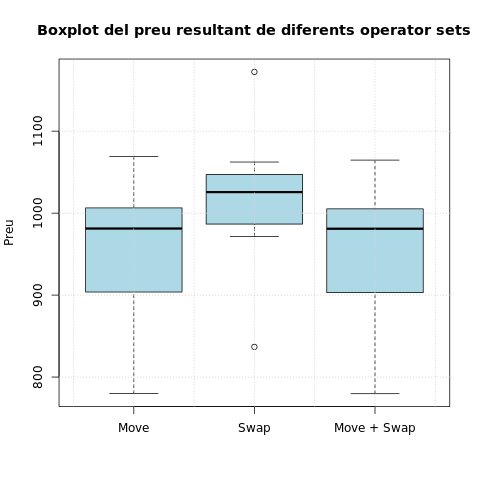
\includegraphics[width=0.45\textwidth]{images/exp1_boxplot.png}
		\caption{Box plot del preu resultant de diferents conjunts d'operadors}
		\label{fig:exp1_boxplot}
	\end{figure}
	
	\begin{table}[H]
		\centering
		\begin{tabular}{|c|c|c|c|c|}
			\hline
			\textbf{Operador} & \textbf{Mediana} & \textbf{Q1} & \textbf{Q3} & \textbf{IQR} \\
			\hline
			Move & 981.245 & 917.275 & 1003.02 & 85.745 \\
			\hline
			Swap & 1025.675 & 992.235 & 1046.285 & 54.05 \\
			\hline
			Move + Swap & 980.87 & 916.525 & 1002.11 & 85.5875\\
			\hline
		\end{tabular}
		\caption{Estadístiques del preu de diferents conjunts d'operadors}
		\label{tab:exp1_estadisticas}
	\end{table}
	
	Com podem observar en la \textit{Figura \ref{fig:exp1_boxplot}}, el resultat obtingut amb l'operador \textit{swap} dista molt dels altres. Així que serà el primer que comentarem. Per començar, cal entendre que amb només un \textit{swap} no recorrerem tot l'espai de cerca per un simple motiu: una oferta de transport que inicialment tingui un paquet assignat mai més podrà estar buida. Aquesta limitació es reflecteix en una mediana major. Podem consultar les dades numèriques de l'experiment a la \textit{Taula \ref{tab:exp1_estadisticas}}. A més, veiem que el rang interquartílic (IQR) amb \textit{swap} és el menor, la qual cosa indica que aquest operador ens proporciona resultats consistents, però no els millors. \\
	
	Per altra banda, observem que els resultats de \textit{move} i \textit{move + swap} són molt similars. Això implica que amb el \textit{move} podem explorar la gran majoria de l'espai de cerca, ja que no té la restricció que presenta l'altre operador. En aquest cas, la única limitació que tindríem es donaria quan volguéssim fer un \textit{swap} de dos paquets. Amb l'operador de \textit{move}, aquest procés s'ha de realitzar en dues operacions com a norma general; però, si un dels paquets no hi càpiga en l'altra oferta, necessitarem tres operacions, utilitzant una oferta auxiliar per assignar temporalment aquell paquet. \\
	
	En casos puntuals, seria probable que no poguéssim fer aquest swap només amb el \textit{move}. Aquest escenari s'ha donat durant els experiments, ja que en alguns casos hem observat una diferència molt petita en el cost, ja que el \textit{swap} ha pogut complementar el que el \textit{move} no podia. Per aquesta raó, els dos conjunts d'operadors ($C_2$ i $C_3$) que estem analitzant presenten resultats similars, però el conjunt que inclou l'operador \textit{swap} obté resultats lleugerament millors en alguns casos. \\
	
	Respecte a la nostra hipòtesi inicial, observem que s'ha complert, ja que el conjunt d'operadors que inclou tant \textit{move} com \textit{swap} ha mostrat un rendiment lleugerament superior en alguns casos. No obstant això, no esperàvem una similitud tan notable entre els resultats obtinguts amb els conjunts d'operadors $C_{\texttt{2}}$ i $C_{\texttt{3}}$. Aquesta similitud indica que l'operador \textit{swap} pot no ser essencial per millorar significativament els resultats en la majoria dels escenaris analitzats. \\
	
	A partir d'aquesta observació, podríem considerar l'opció de reduir el factor de ramificació eliminant l'operador \textit{swap} del conjunt d'operadors utilitzats. La raó darrere d'aquesta decisió es fonamenta en el principi d'eficiència: simplificar el conjunt d'operadors pot conduir a una reducció del temps de càlcul i a una millora en la velocitat d'exploració de l'espai de cerca. \\
	
	En resum, els resultats indiquen que, tot i que el \textit{swap} aporta certes millores en situacions particulars, la seva presència no és extremadament rellevant. Això suggereix que una aproximació més eficient podria ser treballar exclusivament amb l'operador \textit{move}, permetent-nos explorar l'espai de cerca de manera més àgil i reduint potencialment el factor de ramificació, facilitant així la millora del rendiment global de l'algorisme.
	
	\subsection{Experiment 2: Determinació de Solucions Inicials}
	\label{sec:exp2}
	
	Un altre punt que creiem molt important a l'hora de plantejar aquests problemes és la solució inicial. Una solució inicial de qualitat proporciona un diferent punt de partida per explorar l'espai de solucions, la qual cosa pot conduir a diferents resultats finals, o bé a una diferent velocitat per trobar una solució òptima. \\
	
	En aquest experiment, compararem dues estratègies de generació de solucions inicials per avaluar si hi ha alguna diferència notable en els resultats finals quan es fa servir l'algorisme \textit{Hill Climbing} i els operadors escollits a l'apartat anterior: \textit{swap} i \textit{move}.\\
	
	Les dues estratègies que considerarem per la generació de l'estat inicial són:
	
	\begin{itemize}
		\item \emph{Solució Inicial 1}: aquesta és una estratègia que genera solucions inicials amb una qualitat més alta, és a dir, busquem des d'un principi una solució més propera a la que creiem la solució final, més òptima, ja que intentem fer una assignació de paquets a ofertes amb el menor preu possible (\ref{sec:GenSolIni_felicitat}).
		
		\item \emph{Solució Inicial 2}: aquesta estratègia simplement pretén assignar els paquets a ofertes i en cap moment dona prioritat a les ofertes més barates, és per això que està més lluny de la solució final que busquem, però és més ràpida i simple de generar que la primera (\ref{sec:GenSolIni_dia}).
	\end{itemize}
	
	\begin{table}[ht]
		\centering
		\begin{tabular}{|l|p{10cm}|}
			\hline
			Observació & La solució inicial triada pot portar a una millor solució final. \\
			\hline
			Plantejament & Observem la influència de dues solucions inicials en la qualitat de la solució final. \\
			\hline
			Hipòtesi & Una solució inicial menys òptima, la \textit{Solució inicial 2}, proporcionarà significativament millors resultats.\\
			\hline
			Mètode & 
			\begin{itemize}
				\item Agafarem un conjunt de $10$ llavors aleatòries.
				\item Establirem els algorismes \textit{Hill Climbing} per un problema amb 100 paquets i una proporció de pes transportable per les ofertes d'1,2.
				\item Executarem els 10 experiments amb la \textit{Solució inicial 1} i la \textit{Solució inicial 2}, un per cada llavor.
				\item Mesurarem els resultats i n'extraurem conclusions.
			\end{itemize} \\
			\hline
		\end{tabular}
		\label{tab:exp2_apartats}
	\end{table}
	
	Els resultats, que es poden trobar al path \texttt{./Latex/spreadsheets/exp2.csv} de \textit{GitHub} (vegeu l'annex \ref{sec:annex} per accedir-hi), es poden resumir amb el gràfic i la taula que hi ha a continuació:
	
	\begin{figure}[H]
		\centering
		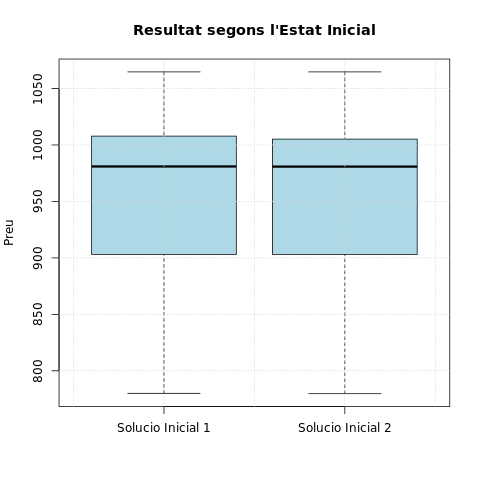
\includegraphics[width=0.45\textwidth]{images/exp2_boxplot.png}
		\caption{Boxplot del preu resultant segons la solució inicial}
		\label{fig:exp2_boxplot}
	\end{figure}
	
	\begin{table}[H]
		\centering
		\begin{tabular}{|c|c|c|c|c|}
			\hline
			\textbf{Operador} & \textbf{Mediana} & \textbf{Q1} & \textbf{Q3} & \textbf{IQR} \\
			\hline
			Solució 1 & 980.975 & 916.58 & 1004.178 & 87.5975 \\
			\hline
			Solució 2 & 980.87 & 916.525 & 1002.112 & 85.5875 \\
			\hline
		\end{tabular}
		\caption{Estadístiques del preu segons la solució inicial}
		\label{tab:exp2_estadisticas}
	\end{table}
	
	Com clarament veiem a la \textit{Figura \ref{fig:exp2_boxplot}} i \textit{Taula \ref{tab:exp2_estadisticas}}, les diferències entre els resultats obtinguts segons les solucions inicials donades són mínimes, tant en la mediana com en el rang interquartílic (IQR). La \textit{Solució inicial 1}, és a dir, la més "òptima", presenta una mediana del preu lleugerament superior ($980.975$ comparada amb $980.87$), però la diferència no és significativa. El rang interquartílic és també lleugerament més ampli per aquesta solució, amb un IQR de $87.60$ en comparació amb els $85.59$ de l'altra solució inicial.\\
	
	Aquestes similituds porten a pensar que ambdues estratègies acaben atrapades en mínims locals, independentment de la qualitat de la solució inicial, per això les diferències en els resultats finals són gairebé inexistents en l'algorisme de \textit{Hill Climbing}, és a dir, totes dues estratègies portaran cap a resultats similars.\\
	
	Després d'analitzar els resultats, podem concloure que no hi ha una diferència significativa entre les dues estratègies de generació de solucions inicials. Això ens dona a pensar que almenys en aquest escenari, l'algorisme \textit{Hill Climbing} tendeix a quedar-se en mínims locals, independentment de la qualitat de la solució inicial. Per tant, pels pròxims experiments, optarem per la generació de solucions inicials menys òptimes, és a dir, per la \textit{Solució inicial 2} \ref{sec:GenSolIni_dia}, ja que simplifica el procés de generar l'Estat Inicial i no empitjora la solució final, de fet, la millora molt lleugerament.
	
	\subsection{Experiment 3: Determinació de paràmetres del \textit{Simulated Annealing}}
	\label{sec:exp3}
	
	L'algorisme de \textit{Simulated Annealing} tal com està implementat accepta els paràmetres: nombre total d'iteracions, iteracions per cada canvi de temperatura (divisor de l'anterior), paràmetres $k$ i $\lambda$ de la funció d'acceptació d'estats; els quals s'han de determinar experimentalment per tal d'obtenir el millor rendiment possible d'aquest algorisme.\\
	
	Per determinar això, hem establert un nombre d'iteracions prou gran que ens permetrà obviar aquesta variable a l'hora d'extreure conclusions sobre els altres paràmetres.
	
	\begin{table}[ht]
		\centering
		\begin{tabular}{|l|p{10cm}|}
			\hline
			Observació & Depenent dels paràmetres del \textit{Simulated Annealing}, es poden obtenir millors resultats. \\
			\hline
			Plantejament & Escollim diferents paràmetres per l'algorisme i analitzem els resultats obtinguts. \\
			\hline
			Hipòtesi & Hi ha alguna combinació de paràmetres pel \textit{Simulated Annealing} que dona millors resultats que altres.\\
			\hline
			Mètode &
			\begin{itemize}
				\item Agafarem un conjunt de $10$ llavors aleatòries.
				\item Establirem l'algorisme \textit{Simulated Annealing} per un problema amb 100 paquets i una proporció de pes transportable per les ofertes d'$1.2$. El nombre d'iteracions el deixarem fix a $100$ i la solució inicial que donarem serà la \textit{Solució inicial 2} (\ref{sec:GenSolIni_dia}), triada a l'experiment anterior \textit{Experiment 2} (\ref{sec:exp2}).
				\item Executarem els $50$ experiments amb cada conjunt de $k=\{1, 5, 25, 125\}$ i $\lambda = \{1, 0.01, 0.0001\}$.
				\item Cadascun d'aquests experiments l'executarem amb diversos valors d'\textit{Steps}, començant per $1$ i augmentant progressivament fins a $1500$, $\{1, 100, 200, 500, ... , 90000, 100000\}$. 
				\item Mesurarem els resultats i n'extraurem conclusions.
			\end{itemize} \\
			\hline
		\end{tabular}
		\label{tab:exp3_apartats}
	\end{table}
	
	Tots els resultats, estan a \texttt{./Latex/spreadsheets/exp3.csv} de \textit{GitHub}, vegeu l'annex \ref{sec:annex}. Aquests resultats es poden simplificar amb l'ajuda del gràfic i la taula que hi ha a continuació. Fixeu-vos que l'eix de les Y no comença a 0, està fet així perquè es puguin veure millor les diferències, ja que el cost de 100 paquets és prou alt i no s'aprecien les diferències si partim de l'origen:
	
	\begin{figure}[H]
		\centering
		\begin{minipage}{0.45\textwidth}
			\centering
			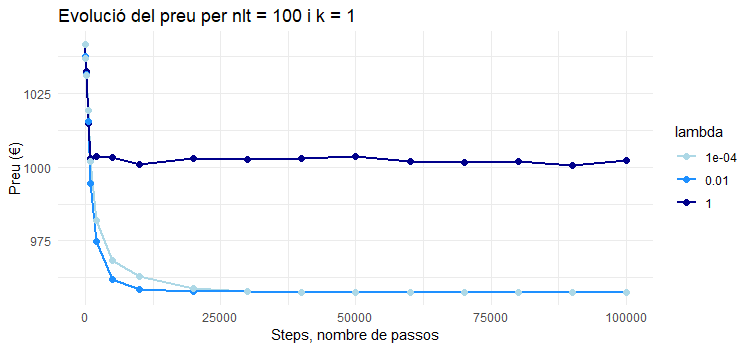
\includegraphics[width=\textwidth]{images/exp3_k1.png}
			\caption{Evolució del preu resultant amb $k=1$ i per $\lambda = {1, 0.01, 0.0001}$, en funció dels \textit{steps}}
			\label{fig:exp3_k1}
		\end{minipage}%
		\hspace{0.05\textwidth} % Espacio entre las figuras
		\begin{minipage}{0.45\textwidth}
			\centering
			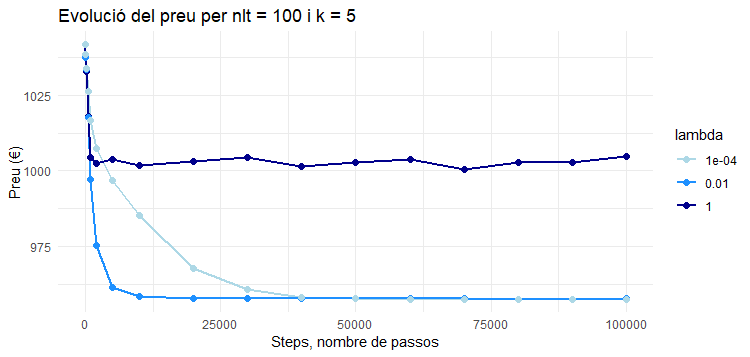
\includegraphics[width=\textwidth]{images/exp3_k5.png}
			\caption{Evolució del preu resultant amb $k=5$ i per $\lambda = {1,0.01,0.0001}$, en funció dels \textit{steps}}
			\label{fig:exp3_k5}
		\end{minipage}
	\end{figure}
	
	\begin{figure}[H]
		\centering
		\begin{minipage}{0.45\textwidth}
			\centering
			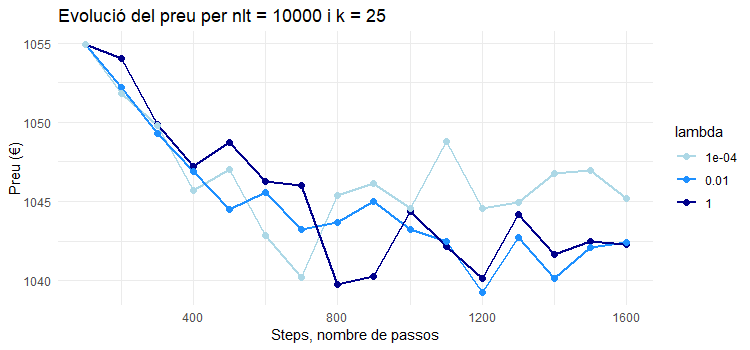
\includegraphics[width=\textwidth]{images/exp3_k25.png}
			\caption{Evolució del preu resultant amb $k=25$ i per $\lambda = {1, 0.01, 0.0001}$, en funció dels \textit{steps}}
			\label{fig:exp3_k25}
		\end{minipage}%
		\hspace{0.05\textwidth} % Espacio entre las figuras
		\begin{minipage}{0.45\textwidth}
			\centering
			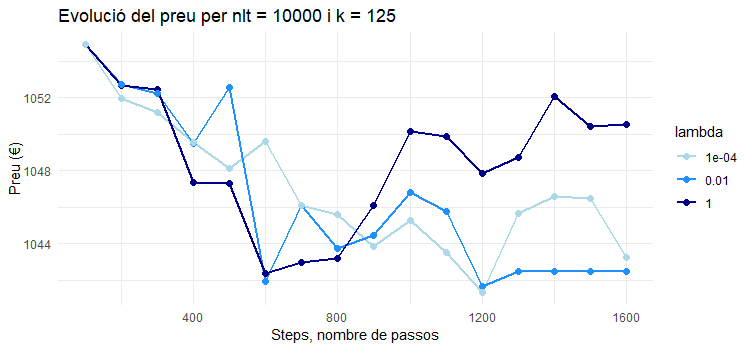
\includegraphics[width=\textwidth]{images/exp3_k125.png}
			\caption{Evolució del preu resultant amb $k=125$ i per $\lambda = {1,0.01,0.0001}$, en funció dels \textit{steps}}
			\label{fig:exp3_k125}
		\end{minipage}
	\end{figure}
	
	\begin{table}[H]
		\centering
		\begin{tabular}{|c|c|c|c|c|}
			\hline
			\textbf{Operador} & \textbf{k=1} & \textbf{k=5} & \textbf{k=25} & \textbf{k=125} \\
			\hline
			$\lambda$=1 & 1009.244 & 1009.888 & 1010.927 & 1011.091 \\
			\hline
			$\lambda$=0.01 & 977.984 & 978.359 & 979.316 & 980.069 \\
			\hline
			$\lambda$=0.0001 & 979.634 & 986.378 & 994.474 & 1001.120 \\
			\hline
		\end{tabular}
		\caption{Mitjana del preu segons el valor de $k$ i $\lambda$, indepent del valor d'\textit{Steps}.}
		\label{tab:exp3_estadisticas}
	\end{table}
	
	Quan analitzem totes les mitjanes, a la \textit{Taula \ref{tab:exp3_estadisticas}}, podem veure que és pels valors més baixos de $lambda$ quan obtenim costos una mica menors. En canvi, respecte la $k$ no sempre obtenim aquests resultats, ja que canviar aquest paràmetre no ha alterat tant el cost resultant i les diferències no són gaire significatives entre aquests valors. \\
	
	Si analitzem per altra banda les gràfiques, podem arribar a la mateixa conclusió. De fet, també ens serveix per analitzar l'evolució dels resultats en funció del valor que li donem a la variable \textit{Steps}. Es pot veure que, en general, com més gran sigui aquesta variable, més baix és el cost, seguint una baixada força constant quan arribem a un cert punt. \\
	
	Podem veure amb els gràfics que per valors de $lambda$ més petits, especialment per $lambda=0.0001$, es necessiten més \textit{steps} per arribar a un cost més estable. A més, aquest valor de lambda necessita més \textit{steps} amb valors de $k$ més alts, com es pot veure a la \textit{Figura \ref{fig:exp3_k125}}. Per això, depenent dels valors triats per la $k$ i $\lambda$, pot ser més recomanable triar un valor d'\textit{steps} o un altre, en funció dels valors de costos i eficiència que busquem. \\
	
	Com els resultats són força semblants pels diferents valors de $k$, però per $lambda$ veiem que ens interessen valors més petits, triem una opció amb valors de $k$ i $\lambda$ baixos, com per exemple k=1, $\lambda=0.01$. Un cop triat això, si ens fixem en el gràfic \textit{Figura \ref{fig:exp3_k1}}, i ens fixem en el cost resultant en funció dels \textit{steps}, veiem que un valor de $steps=20000$ ja és més que suficient per assegurar-nos un resultat favorable tenint en compte també valors d'eficiència. \\
	
	Per tant, el paràmetres que triem per \textit{Simulated Annealing} i que es faran servir per propers experiments és: k=1, $\lambda = 0.01$ i $steps = 20000$.
	
	
	\subsection{Experiment 4: Anàlisi del temps d'execució}
	\label{sec:exp4}
	
	Un cop hem experimentat amb els diversos factors que influeixen en la cerca d'una solució òptima al problema i hem determinat quins funcionen millor, ens interessa ara també veure com evoluciona el temps d'execució per trobar una solució per veure si és factible trobar-ho en un temps raonable.\\
	
	L'objectiu és analitzar com evoluciona el temps d'execució necessari per trobar una solució utilitzant l'algorisme de \textit{Hill Climbing}, en funció de dos factors clau: el nombre de paquets a enviar i la proporció de pes transportable per les ofertes. \\
	
	L'escenari és el mateix que en els experiments anteriors: treballem amb la generadora d'una solució inicial d'entrega al dia (\ref{sec:GenSolIni_dia}), la funció heurística que només té en compte els costos, el conjunt d'operadors tindrà \textit{swap} i \textit{moure}. Tots aquests experiments han estat seleccionats mitjançant els experiments anteriors (\ref{sec:exp1}, \ref{sec:exp2}). Aquest cop, el focus es desplaça cap a l'anàlisi de la complexitat temporal del sistema, estudiant com es veu afectat el temps d'execució quan variem els dos paràmetres mencionats. \\
	
	Com que tenim dos factors a estudiar, dividim aquest experiment en dues parts:
	
	\begin{itemize}
		\item \emph{Impacte de la proporció del pes transportable}: es fixarà el nombre de paquets a $100$ i s'anirà augmentant la proporció del pes transportable des de $1.2$ en increments de $0.2$ on volem identificar com la relació entre la capacitat de les ofertes i el pes dels paquets afecta el rendiment de l'algorisme.
		
		\item \emph{Impacte del nombre de paquets}: es fixarà la proporció del pes transportable a $1.2$ i es variarà el nombre de paquets, començant per $100$ i augmentant-lo de $50$ en $50$. S'analitzarà com l'increment en la quantitat de paquets afecta el temps d'execució.
		
	\end{itemize}
	
	\subsubsection{Proporció del pes transportable}
	\begin{table}[ht]
		\centering
		\begin{tabular}{|l|p{10cm}|}
			\hline
			Observació & Com afecta la proporció del pes transportable al temps d'execució per trobar solucions òptimes.\\
			\hline
			Plantejament & Analitzarem l'impacte d'augmentar la proporció del pes transportable sobre el temps d'execució. \\
			\hline
			Hipòtesi & Es preveu que a mesura que augmenta la proporció del pes transportable, el temps d'execució s'incrementi, ja que amb una capacitat més gran de les ofertes, l'espai de cerca creix.\\
			\hline
			Mètode &
			\begin{itemize}
				\item Agafarem un conjunt de $10$ llavors aleatòries.
				\item Establirem els algorismes \textit{Hill Climbing} per un problema amb 100 paquets, amb la funció heurística que minimitza només costos i amb el generador de solucions aleatori.
				\item Executarem $10$ experiments per a cada una de les proporcions de pes transportable $\{1.2, 1.4, 1.5, 1.6, 1.8, 2.0 \}$, un per cada llavor.
				\item Mesurarem els resultats i n'extraurem conclusions.
			\end{itemize} \\
			\hline
		\end{tabular}
		\label{tab:exp4a_apartats}
	\end{table}
	
	Els resultats dels experiments realitzats es poden trobar al path \texttt{./Latex/spreadsheets/exp4a.csv} de \textit{GitHub}, vegeu l'annex \ref{sec:annex}. Podem veure els resultats representats en els gràfics que hi ha a continuació. En el primer gràfic de la \textit{Figura \ref{fig:exp4a_grafic_lineal}} s'ha fet la mitjana dels temps de totes les llavors que s'han escollit per cada valor de proporció del pes transportable triats.
	
	\begin{figure}[H]
		\centering
		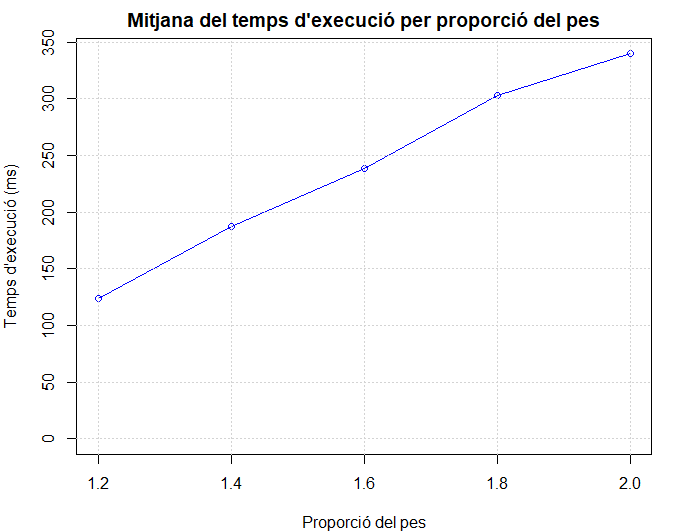
\includegraphics[width=0.45\textwidth]{images/exp4a_grafic_lineal.png}
		\caption{Gràfic del temps d'execució de l'algorisme en funció del nombre de paquets}
		\label{fig:exp4a_grafic_lineal}
	\end{figure}
	
	\begin{table}[H]
		\centering
		\begin{tabular}{|c|c|c|}
			\hline
			\textbf{Proporció del pes} & \textbf{MedianaTemps} & \textbf{MitjanaTemps} \\
			\hline
			1.2 & 118.3 & 123.74\\
			\hline
			1.4 & 187.9 & 186.96\\
			\hline
			1.6 & 239.4 & 238.6\\
			\hline
			1.8 & 284 & 302.8\\
			\hline
			2.0 & 334.9 & 339.7\\
			\hline
		\end{tabular}
		\caption{Estadístiques del temps d'execució en mil·lisegons en funció de la proporció del pes}
		\label{tab:exp4a_taula}
	\end{table}
	
	En la \textit{Figura \ref{fig:exp4a_grafic_lineal}} es pot apreciar que el temps d'execució de l'algorisme de \textit{Hill Climbing} va augmentant de forma proporcional a la que ho fa la proporció del pes transportable; és a dir que s'aproxima a un creixement lineal la funció obtinguda. \\
	
	Dels dos operadors utilitzats, només el de \textit{move} té un factor de ramificació que depèn del nombre d'ofertes, sent de l'ordre de $O(n \cdot m)$, on $m$ és el nombre d'ofertes. En incrementar el nombre d'ofertes, també augmenta l'espai de cerca a causa del factor de ramificació d'aquest operador, de manera que buscar en un espai més gran evidentment triga més. Com que el nombre d'ofertes no té cap exponent, és raonable esperar aquest comportament lineal en el temps d'execució.
	
	\subsubsection{Nombre de paquets}
	\label{sec:exp4b_nombrePaq}
	
	\begin{table}[ht]
		\centering
		\begin{tabular}{|l|p{10cm}|}
			\hline
			Observació & Com afecta el nombre de paquets al temps d'execució per trobar solucions òptimes. \\
			\hline
			Plantejament & Analitzarem l'impacte d'augmentar el nombre de paquets sobre el temps d'execució.\\
			\hline
			Hipòtesi & Es preveu que a mesura que augmenta el nombre de paquets, el temps d'execució també augmenti, ja que el problema es torna més complex en gestionar un nombre més gran de paquets.\\
			\hline
			Mètode &
			\begin{itemize}
				\item Agafarem un conjunt de $10$ llavors aleatòries.
				\item Establirem els algorismes \textit{Hill Climbing} per un problema amb la proporció del pes de transport fixat  $1,2$, amb la funció heurística que minimitza només costos i amb el generador de solucions aleatori.
				\item Executarem $10$ experiments per a cada nombre de paquets \{100, 150, 200, 250, 300, 350, 400 \}, un per cada llavor.
				\item Mesurarem els resultats i n'extraurem conclusions.
			\end{itemize} \\
			\hline
		\end{tabular}
		\label{tab:exp4b_apartats}
	\end{table}
	
	Els resultats dels experiments realitzats, que es poden trobar al \textit{path} \texttt{./Latex/spreadsheets/exp4b.csv} de \textit{GitHub} (vegeu l'annex \ref{sec:annex} per accedir-hi), els podem veure representats en els gràfics que hi ha a continuació. En el primer gràfic de la \textit{Figura \ref{fig:exp4b_grafic_lineal2}} s'ha fet la mitjana dels temps de totes les llavors que s'han escollit per cada valor de nombre de paquets triats; la \textit{Figura \ref{fig:exp4b_boxplots}} conté un box plot per cada nombre de paquets amb els temps d'execució.\\
	
	\begin{figure}[H]
		\centering
		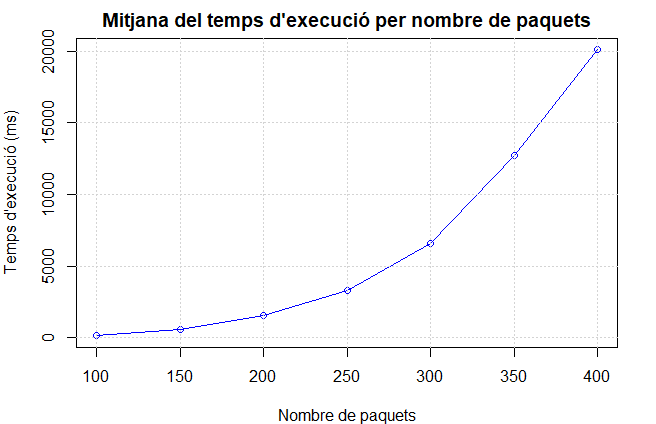
\includegraphics[width=0.45\textwidth]{images/exp4b_grafic_lineal2.png}
		\caption{Gràfic del temps d'execució de l'algorisme en funció del nombre de paquets}
		\label{fig:exp4b_grafic_lineal2}
	\end{figure}
	
	\begin{figure}[H]
		\centering
		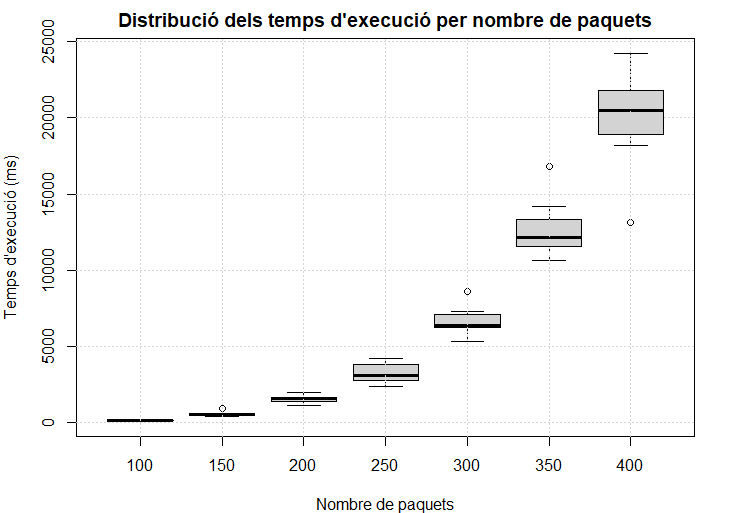
\includegraphics[width=0.45\textwidth]{images/exp4b_boxplots.png}
		\caption{Boxplots dels temps d'execució per cada valor de nombre de paquets}
		\label{fig:exp4b_boxplots}
	\end{figure}
	
	\begin{table}[H]
		\centering
		\begin{tabular}{|c|c|c|}
			\hline
			\textbf{Nombre paquets} & \textbf{MedianaTemps} & \textbf{MitjanaTemps} \\
			\hline
			100 & 140.6 & 134.165\\
			\hline
			150& 529.2 & 570.7\\
			\hline
			200& 1604.8 & 1549.34\\
			\hline
			250& 3099.4 & 3277.24\\
			\hline
			300& 6362.7 & 6591.74\\
			\hline
			350& 12133.8 & 12695.88\\
			\hline
			400& 20456.6 & 20087.64\\
			\hline
		\end{tabular}
		\caption{Estadístiques del temps d'execució en mil·lisegons en funció del nombre de paquets}
		\label{tab:exp4b_temps}
	\end{table}
	
	Com es pot observar en la \textit{Figura \ref{fig:exp4b_grafic_lineal2}}, la mitjana dels temps d'execució augmenta de manera significativa a mesura que creix el nombre de paquets a assignar en el problema d'optimització. Contràriament a un creixement lineal, el comportament observat en el gràfic s'ajusta millor a una funció polinòmica de grau superior a $1$. Aquesta observació confirma la nostra hipòtesi inicial, que preveia un augment no lineal del temps d'execució a mesura que augmentava la complexitat del problema. \\
	
	A més de la mitjana, la \textit{Figura \ref{fig:exp4b_boxplots}} presenta la distribució dels temps d'execució mitjançant un box plot, que ens proporciona una visió detallada de la variabilitat dels resultats en funció del nombre de paquets. Aquí es pot observar clarament que, per a valors més petits de nombre de paquets $\in [100, 200]$, la variabilitat és baixa, amb distribucions ajustades i valors consistents entre diferents execucions. No obstant això, a partir de $250$ paquets, la dispersió augmenta notablement, indicant una major variabilitat en els temps d'execució. Això podria indicar que, en casos amb més paquets, hi ha més variabilitat en el temps necessari per trobar la solució òptima, depenent de la llavor inicial i l'exploració de l'espai de cerca. \\
	
	El creixement quadràtic observat es pot explicar per la naturalesa dels operadors utilitzats en l'algorisme de \textit{Hill Climbing}. Degut al factor de ramificació inherent dels operadors, el qual és de l'ordre de $O(n^2)$, l'espai de cerca s'expandeix de forma quadràtica amb l'increment del nombre de paquets. Així, cada cop que es creix el nombre de paquets, l'algorisme ha d'explorar un espai de solucions molt més gran, la qual cosa resulta en un augment substancial del temps necessari per trobar una solució òptima. Aquesta complexitat quadràtica és típica dels algorismes que han de tractar amb grans espais de cerca, i fa que el temps d'execució s'incrementi ràpidament en problemes d'aquesta magnitud, tal com es reflecteix en el gràfic de la mitjana com en el box plot. \\
	
	A partir de la \textit{Taula \ref{tab:exp4b_temps}}, on es mostren els temps d'execució per diferents nombres de paquets, podem observar un creixement substancial a mesura que el nombre de paquets augmenta. La mediana i la mitjana dels temps d'execució reflecteixen aquesta tendència, confirmant la complexitat quadràtica de l'algorisme amb el factor de ramificació $O(n^2)$, tal com s'ha discutit anteriorment. \\
	
	En conclusió, d'acord amb la hipòtesi plantejada s'ha observat que el temps d'execució de l'algorisme de \textit{Hill Climbing} per trobar una solució a un problema donat augmenta de forma no lineal en funció del nombre de paquets a assignar; la variabilitat de temps també incrementa. En comparació amb l'experiment anterior on s'ha vist que el creixement del temps era lineal, aquí ens trobem amb un creixement quadràtic en contrast; resultats que es justifiquen analitzant els factors de ramificació dels operadors implementats a l'algorisme utilitzat. Amb aquests dos experiments s'ha pogut observar la importància del factor de ramificació, el qual s'ha de tenir en consideració a l'hora d'escollir uns bons operadors. \\
	
	Com a puntualització extra, com s'ha esmentat en el \textit{Experiment 1 (\ref{sec:exp1})}, podríem obviar de l'operador \textit{swap}, ja que no ens ofereix una millora gaire notable. Aconseguint, d'aquesta manera, que l'increment de temps passi a ser lineal, ja que l'operador \textit{move} ho és, i seria l'únic que utilitzaríem. \\
	
	
	\subsection{Experiment 5: Influència de la proporció de les ofertes}
	
	Un altre factor que es vol analitzar és com influeix l'augment de la proporció de les ofertes en el comportament dels costos de transport i emmagatzematge en el problema. En concret, volem determinar si incrementar el nombre de ofertes disponibles millora de manera significativa els costos totals dels paquets i si realment mereix la pena augmentar les ofertes. \\
	
	Els costos de transport es veuran influenciats principalment per la capacitat de les ofertes per ajustar-se de manera eficient al pes i nombre de paquets a enviar, mentre que el cost d'emmagatzematge dependrà de la efectivitat de l'assignació dels paquets a ofertes que triguin poc. És necessari investigar fins a quin punt l'augment del nombre d'ofertes continua sent beneficiós. \\
	
	Aprofitant el mateix experiment on veiem el comportament del temps d'execució en funció de la proporció del pes transportable a l'apartat \ref{sec:exp4b_nombrePaq}, amb les mateixes llavors i condicions, només que ara ens enfocarem amb els resultats obtinguts sobre els costos de transport i emmagatzematge.
	
	\begin{table}[H]
		\centering
		\begin{tabular}{|l|p{10cm}|}
			\hline
			Observació & Com afecta la proporció del pes transportable al costos totals per trobar solucions òptimes.\\
			\hline
			Plantejament & Analitzarem l'impacte d'augmentar la proporció del pes transportable sobre el costos de transport i emmagatzematge. \\
			\hline
			Hipòtesi & A mesura que augmenta la proporció del pes transportable, els costos disminueixin, ja que amb una capacitat més gran de les ofertes, es podran trobar ofertes millor a assignar als paquets.\\
			\hline
			Mètode &
			\begin{itemize}
				\item Agafarem un conjunt de $10$ llavors aleatòries.
				\item Establirem els algorismes \textit{Hill Climbing} per un problema amb 100 paquets, amb la funció heurística que minimitza només costos i amb el generador de solucions aleatori.
				\item Executarem $10$ experiments per a cada una de les proporcions de pes transportable $\{1.2, 1.4, 1.5, 1.6, 1.8, 2.0 \}$, un per cada llavor.
				\item Mesurarem els resultats i n'extraurem conclusions.
			\end{itemize} \\
			\hline
		\end{tabular}
		\label{tab:exp5_apartats}
	\end{table}
	
	Ja amb els experiment executats, hem col·locat els resultats al projecte \textit{GitHub} (vegeu l'annex \ref{sec:annex} per accedir-hi), en el \textit{path} \texttt{./Latex/spreadsheets/ex6.csv} i \texttt{./Latex/spreadsheets/ex5.csv}. A partir d'aquestes dades hem fet extret un gràfic representatiu dels resultats i un altre amb box plots dels preus per cada proporció de pes transportable.
	
	\begin{figure}[H]
		\centering
		\begin{minipage}{0.45\textwidth}
			\centering
			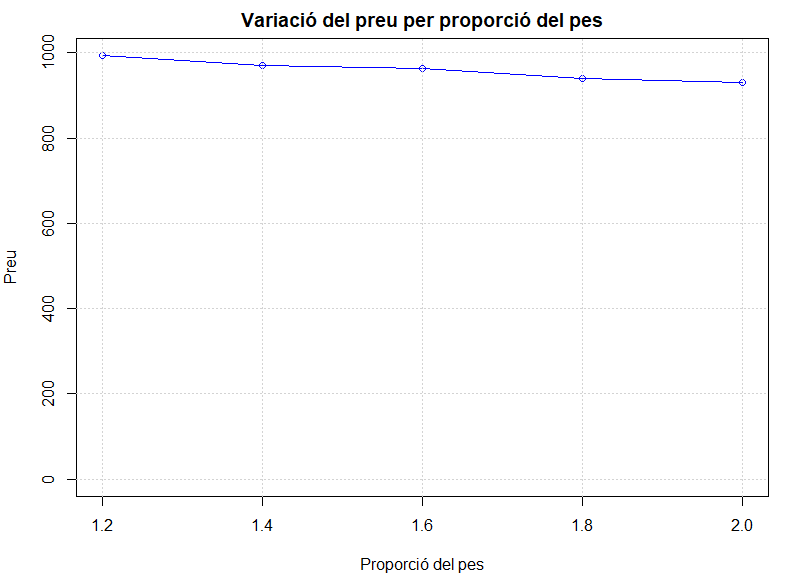
\includegraphics[width=\textwidth]{exp5_grafic_lineal.png}
			\caption{Gràfic de la mitjana dels costos totals per cada valor de nombre de paquets}
			\label{fig:exp5_grafic_lineal}
		\end{minipage}\hfill
		\begin{minipage}{0.45\textwidth}
			\centering
			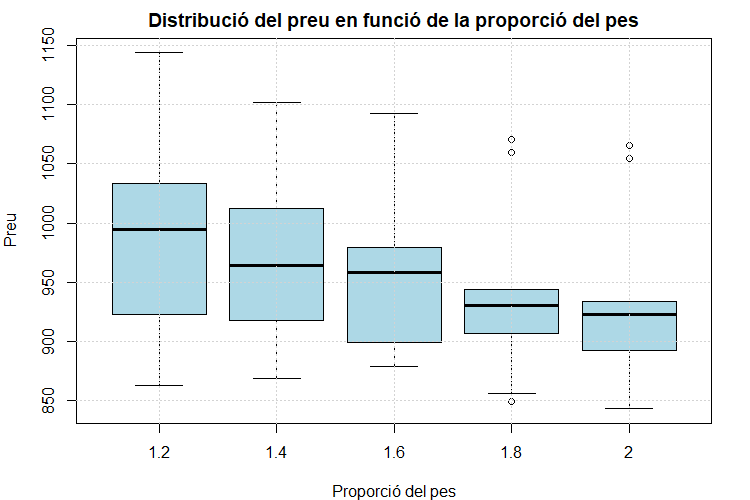
\includegraphics[width=\textwidth]{images/exp5_boxplot.png}
			\caption{Boxplots dels costos totals per cada valor de nombre de paquets}
			\label{fig:exp5_boxplot}
		\end{minipage}
	\end{figure}
	
	
	Els resultats mostren una tendència general a la disminució del cost total quan s'augmenten les ofertes, encara que aquesta disminució no és dràstica ni exponencial, sinó més aviat lineal i moderada. És a dir, a mesura que s'incrementa el nombre d'ofertes, el sistema aconsegueix optimitzar millor l'assignació dels paquets, degut segurament a que apareguin més ofertes que ofereixin un preu de transport més barat per a una entrega determinada de dies o que tingui més capacitat per transportat; és a dir hi ha més on escollir, la qual cosa redueix els costos d'emmagatzematge i transport, però sense una millora desproporcionada. En uns certs casos, incrementar lleugerament el nombre d'ofertes no genera millores significatives en el cost, i fins i tot en alguns escenaris a penes s'observa una diferència respecte a tenir un nombre menor d'ofertes. \\
	
	D'altra banda, cal destacar que augmentar lleugerament el nombre d'ofertes no sempre genera una millora significativa en el cost total; en alguns casos, els canvis són mínims o fins i tot inexistents. No obstant això, quan l'augment d'ofertes és prou significatiu, sí que s'observa una millora apreciable en l'optimització del sistema. A nivell global, encara que els increments petits no sempre impactin de manera clara, quan s'afegeix un nombre considerable d'ofertes, la reducció del cost de transport i emmagatzematge es torna més notable, reflectint una optimització més efectiva del procés. \\
	
	En resum, encara que augmentar el nombre d'ofertes és una estratègia vàlida per a reduir els costos, no sempre és eficient més enllà d'un cert punt. Perquè aquesta estratègia sigui efectiva, és necessari augmentar les ofertes de manera significativa, ja que increments marginals no generen millores importants. A més, l'impacte varia segons l'escenari, la qual cosa indica que l'optimització del sistema no depèn únicament de la quantitat d'ofertes, sinó també de com estan estructurades i com interactuen amb les característiques del problema. \\
	
	A nivell global, encara que els increments petits no sempre impactin de manera clara, quan s'afegeix un nombre considerable d'ofertes, la reducció del cost de transport i emmagatzematge es torna més notable, i a més qualsevol disminució dels costos és beneficiós per a l'empresa.
	
	\subsection{Experiment 6: Influència de la ponderació de la felicitat (HC)}
	
	Un altre punt clau a l'hora de crear algorismes de cerca local és l'heurística. En aquest cas, una de les heurístiques proposades no només té en compte una optimització del preu total de transport i emmagatzematge, sinó que també té en compte l'optimització de la felicitat dels clients. És important saber conèixer quins són els objectius a l'hora de fer la distribució per veure quanta importància es dona a cadascun d'aquests factors, ja que no podem, alhora, minimitzar al màxim el preu i maximitzar la felicitat dels clients. \\
	
	En canvi, creiem que el canvi en la ponderació de la felicitat, no hauria d'alterar gaire el temps d'execució de l'algorisme, ja que el recorregut de solucions que hi ha de fer hauria de ser semblant. \\
	
	Per comprovar tot això, ara avaluarem l'heurística per veure quanta influència té la felicitat en el preu resultant, variant la ponderació de la felicitat en aquesta. Per veure això, farem servir l'algorisme de \textit{Hill Climbing}, amb un enviament de 100 paquets i una proporció de pes transportable per les ofertes d'$1.2$.
	
	\begin{table}[H]
		\centering
		\begin{tabular}{|l|p{10cm}|}
			\hline
			Observació & Creiem que si volem augmentar la felicitat dels nostres clients, també hi haurà un augment del cost total. Però en canvi, això no influirà en el temps d'execució. \\
			\hline
			Plantejament & Generem diverses solucions variant la ponderació de la felicitat dins l'heurística per veure com influeix en el preu i en el temps d'execució. \\
			\hline
			Hipòtesi & El preu serà més elevat si augmentem la ponderació de la felicitat dins l'heurística, però el temps emprat per trobar la solució serà el mateix. \\
			\hline
			Mètode & 
			\begin{itemize}
				\item Agafarem un conjunt de $10$ llavors aleatòries per cada ponderació de felicitat.
				\item Establirem els algorismes \textit{Hill Climbing}, i generador de solucions pseudo-aleatori, \textit{Solució Inicial 2}.
				\item Executarem l'experiment amb 100 paquets i una proporció d'1,2.
				\item Anirem augmentat de 5 en 5 la felicitat, partint de 0 i arribant fins a 20.
				\item Mesurarem els resultats (preu i temps) i n'extraurem conclusions.
			\end{itemize} \\
			\hline
		\end{tabular}
		\label{tab:exp6_apartats}
	\end{table}
	
	Ja amb els experiment executats, hem col·locat els resultats al projecte \textit{GitHub} (vegeu l'annex \ref{sec:annex} per accedir-hi), en el \textit{path} \texttt{./Latex/spreadsheets/ex6.csv} i \texttt{./Latex/spreadsheets/ex6b.csv}. A partir d'aquestes dades hem fet dos gràfics representatiu dels resultats.
	
	\begin{figure}[H]
		\centering
		\begin{minipage}{0.45\textwidth}
			\centering
			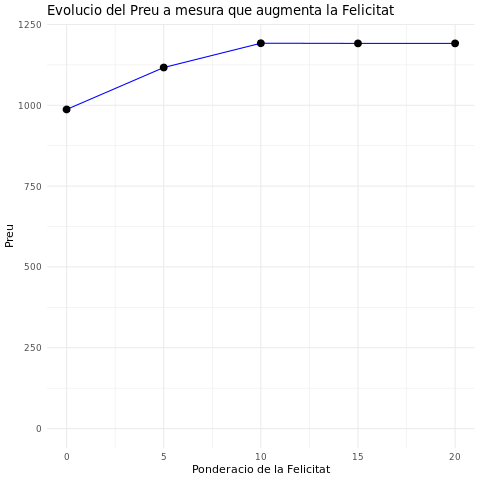
\includegraphics[width=\textwidth]{images/exp6_grafic.png}
			\caption{Gràfic del preu resultant al variar la ponderació de la felicitat}
			\label{fig:exp6a_grafic}
		\end{minipage} \hfill
		\begin{minipage}{0.45\textwidth}
			\centering
			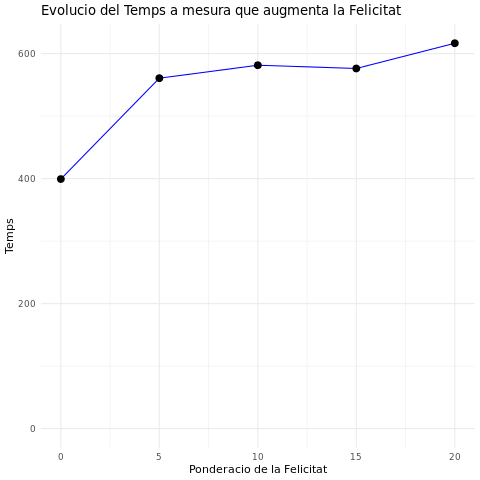
\includegraphics[width=\textwidth]{images/exp6b_grafic.png}
			\caption{Gràfic del temps d'execució al variar la ponderació de la felicitat}
			\label{fig:exp6b_grafic}
		\end{minipage}
	\end{figure}
	
	\begin{table}[H]
		\centering
		\begin{tabular}{|c|c|c|}
			\hline
			\textbf{Ponderació heurística} & \textbf{Mediana} & \textbf{MedianaTemps} \\
			\hline
			$Felicitat \times 0$ & 1010.5 & 396\\
			\hline
			$Felicitat \times 5$ & 1141.105 & 523\\
			\hline
			$Felicitat \times 10$ & 1243 & 535\\
			\hline
			$Felicitat \times 15$ & 1243.5 & 579\\
			\hline
			$Felicitat \times 20$ & 1243.5 & 600\\
			\hline
		\end{tabular}
		\caption{Estadístiques del preu i temps d'execució segons la ponderació de la felicitat}
		\label{tab:exp6_estadisticas}
	\end{table}
	
	Com podem veure a la \textit{Figura \ref{fig:exp6a_grafic}}, la felicitat té una petita influència en el cost final, ja que si comparem la mediana entre quan no tenim en compte la felicitat a l'heurística i quan tenim una ponderació de $20$ dins d'aquesta, veiem que hi ha una diferència d'una mica més de $200$. \\
	
	També podem veure que a mesura que aquesta augmenta, entre els experiments que multipliquen la felicitat per $10$ i els que ho fan per $20$, la diferència és gairebé única. Això és possible que sigui degut a que s'apropa a un mínim local i aquesta ponderació de la felicitat no és tan alta en comparació. \\
	
	Si avaluem ara el temps d'execució en aquests algorismes, vist a la \textit{Figura \ref{fig:exp6b_grafic}}, sí que ens sorprèn trobar-nos un petit augment en aquest a mesura que augmentem la ponderació de la felicitat. Malgrat que aquest també depèn d'altres factors externs a l'algorisme, és possible que això sigui degut a que el ventall de solucions properes quan tenim en compte la felicitat, pot ser major. És a dir, com estem restant la felicitat al cost, hi ha més factors que influeixen al resultat. \\
	
	Com a conclusió, podríem dir que efectivament el preu augmenta amb un increment de la ponderació de la felicitat, però que aquest augment es manté estable arribat a un punt. I, respecte al temps d'execució, aquest sí que pot estar influenciat lleugerament per la ponderació d'aquesta felicitat.
	
	\subsection{Experiment 7: Influència de la ponderació de la felicitat (SA)}
	
	Donat l'escenari de l'experiment anterior, ara el que volem tornar a veure com afecta la felicitat a l'heurística però, aquest cop, amb l'algorisme de \textit{Simulated Annealing}. D'aquesta manera, podrem comparar tots dos algorismes i analitzar si hi ha diferències entre les tendències de tots dos. \\
	
	Per fer això, farem servir els paràmetres de \textit{Simulated Annealing} obtinguts a l'Experiment 3 (\ref{sec:exp3}).
	
	\begin{table}[ht]
		\centering
		\begin{tabular}{|l|p{10cm}|}
			\hline
			Observació & Creiem que si volem augmentar la felicitat dels nostres clients, també hi haurà un augment del cost total. Però en canvi, això no influirà en el temps d'execució. Tot això vist amb \textit{Simulated Annealing}. \\
			\hline
			Plantejament & Generem diverses solucions variant la ponderació de la felicitat dins l'heurística per veure com influeix en el preu i en el temps d'execució. \\
			\hline
			Hipòtesi & El preu serà més elevat si augmentem la ponderació de la felicitat dins l'heurística, però el temps emprat per trobar la solució serà el mateix, i l'evolució d'aquest serà molt semblant al del \textit{Hill Climbing}. \\
			\hline
			Mètode & 
			\begin{itemize}
				\item Agafarem un conjunt de $10$ llavors aleatòries per cada ponderació de felicitat.
				\item Establirem els algorismes \textit{Simulated Annealing}, i generador de solucions pseudo-aleatori, \textit{Solució Inicial 2}.
				\item Executarem l'experiment amb 100 paquets i una proporció d'1,2.
				\item Els paràmetres de \textit{Simulated Annealing} que farem servir són k=1, $\lambda$=0.01, iteracions=100 i steps=20000.
				\item Anirem augmentat de 5 en 5 la felicitat, partint de 0 i arribant fins a 20.
				\item Mesurarem els resultats (preu i temps) i n'extraurem conclusions.
			\end{itemize} \\
			\hline
		\end{tabular}
		\label{tab:exp7_apartats}
	\end{table}
	
	\begin{figure}[H]
		\centering
		\begin{minipage}{0.45\textwidth}
			\centering
			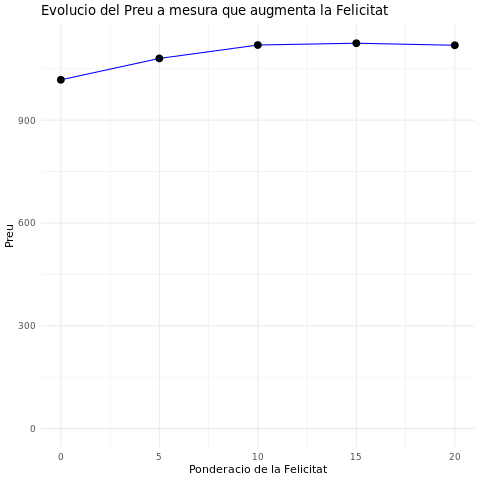
\includegraphics[width=\textwidth]{images/exp7_grafic.png}
			\caption{Gràfic del preu resultant al variar la ponderació de la felicitat}
			\label{fig:exp7_grafic}
		\end{minipage} \hfill
		\begin{minipage}{0.45\textwidth}
			\centering
			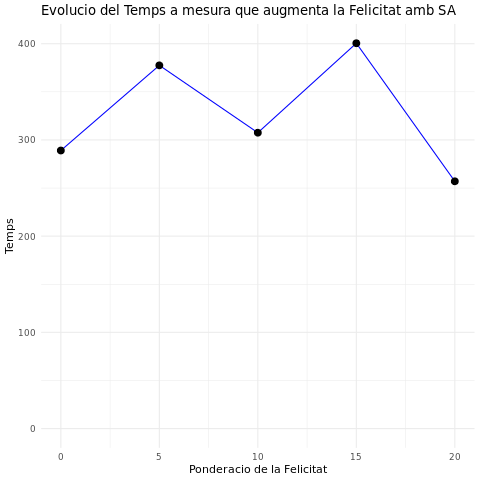
\includegraphics[width=\textwidth]{images/exp7b_grafic.png}
			\caption{Gràfic del temps d'execució al variar la ponderació de la felicitat amb SA}
			\label{fig:exp7b_grafic}
		\end{minipage}
	\end{figure}
	
	\begin{table}[H]
		\centering
		\begin{tabular}{|c|c|c|}
			\hline
			\textbf{Ponderació heurística} & \textbf{Mediana} & \textbf{MedianaTemps} \\
			\hline
			$Felicitat \times 0$ & 1045.66 & 289\\
			\hline
			$Felicitat \times 5$ & 1117.16 & 378\\
			\hline
			$Felicitat \times 10$ & 1162.775 & 308\\
			\hline
			$Felicitat \times 15$ & 1176.16 & 400\\
			\hline
			$Felicitat \times 20$ & 1162.07 & 257\\
			\hline
		\end{tabular}
		\caption{Estadístiques del preu i temps d'execució segons la ponderació de la felicitat}
		\label{tab:exp7_estadisticas}
	\end{table}
	
	Amb aquests resultats podem extreure unes conclusions semblants a les de l'experiment anterior, ja que es veu una petita influència de la felicitat en el cost final. Malgrat que aquesta diferència és una mica menor que quan fèiem servir \textit{Hill Climbing} (100 respecte 200), veiem que la tendència és semblant: comença a l'alça i cap al final es manté constant. \\
	
	Respecte al temps d'execució, es pot veure a la \textit{Figura \ref{fig:exp7b_grafic}} que la ponderació de la felicitat a l'heurística no té una relació directa amb el temps d'execució, ja que aquesta es manté inestable durant les diferents heurístiques. Per tant, aquest no hauria de ser un aspecte a tenir en compte a l'hora de triar l'heurística desitjada. Però, sí que podem dir que aquesta afecta al cost total, especialment si comparem entre les ponderacions nul·les i baixes. \\
	
	
	\subsection{Experiment 8: Influència del preu d'emmagatzematge en les solucions}
	
	\subsubsection{Disminució preu emmagatzematge}
	
	Si fem que el cost d'emmagatzematge sigui més baix, això clarament farà que el cost total disminueixi, ja que aquest té una influència directa en el resultat, sent 0,25€/kg/dia una quantitat considerable. Al tractar-se d'un cost significatiu dins el model, una reducció substancial podria alleugerir considerablement el cost global. Si ens fixem en la felicitat resultant, aquesta és possible que es vegi negativament afectada i que baixi, perquè quan el preu baixa, el cost de mantenir els paquets al magatzem és menor, per la qual cosa tindrà menys pes dins l'heurística; l'algorisme té menys pressió per accelerar l'entrega dels paquets. L'algorisme pot permetre mantenir els paquets més temps en el magatzem sense que impacti massa en el cost total; ja que també les ofertes que entreguen en més dies els paquets acostumen a ser més barats amb les quals és necessari guardar els paquets al magatzem i com a conseqüència els paquets arriben més tard disminuint la felicitat.\\
	
	\subsubsection{Augment preu emmagatzematge}
	
	En canvi, si augmentem aquest cost, és possible que el resultat sigui el contrari, ja que quan el preu puja, té proporcionalment un pes més gran a l'heurística, cosa que per una banda farà que es doni menys importància a la felicitat però. Per l'altra, això incentiva a l'algorisme a intenti tenir els paquets el mínim temps possible al magatzem, perquè mantenir-los allà cada cop serà més costós, per tant, això pot resultar en que s'entregaran els paquets el més aviat possible, el qual augmentarà la felicitat dels usuaris. Però, per altra banda, si tenim en compte que està augmentant una part important de l'heurística, també veiem el cost total augmentarà.\\
	
	
	\subsection{Experiment 9: Especial}
	
	L'eficàcia temporal és un aspecte clau en els algorismes d'intel·ligència artificial. En aquest experiment, per a una entrada donada, extraurem dades sobre el temps necessari perquè l'algorisme s'executi. Els paràmetres que proporcionarem al programa seran: 100 paquets, una proporció de $1.2$ i una llavor de $1234$. A més, utilitzarem el mètode \textit{Hill Climbing} amb els operadors més òptims, que vam examinar en el primer experiment. Aquest conjunt d'operadors inclourà les operacions \textit{move} i \textit{swap}. Només ens falta definir un últim paràmetre: el generador de solucions inicials. Aquest també ha estat seleccionat a partir d'experiments anteriors, més concretament del segon experiment, on vam obtenir els millors resultats amb el generador més 'aleatori'. \\
	
	\begin{figure}[H]
		\centering
		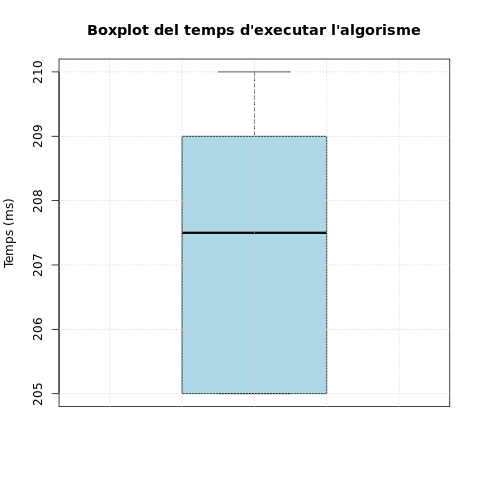
\includegraphics[width=0.45\textwidth]{images/exp9_boxplot.png}
		\caption{Boxplot del temps d'execució}
		\label{fig:exp9_boxplot}
	\end{figure}
	
	A la \textit{Figura \ref{fig:exp9_boxplot}}, observem la distribució dels temps d'execució obtinguts. La mediana és de $207.5$ ms i l'IQR és de $3.5$, cosa que indica que el temps emprat pel programa és força estable. \\
	
	Amb aquests paràmetres, \textit{Hill Climbing} aconsegueix trobar un mínim on l'assignació de paquets té un cost de $794.675$ €.
	
	\subsection{Experiment 10: Comparativa Hill Climbing i Simulated Annealing}
	
	Per comparar els resultats obtinguts amb tots dos algorismes, fets servir al llarg d'aquest treball, farem servir diferents entrades amb 400 paquets i una proporció dels paquets d'1.2, així com també els paràmetres pel \textit{Simulated Annealing} obtinguts a l'experiment 3(\ref{sec:exp3}).
	
	\begin{figure}[H]
		\centering
		\begin{minipage}{0.45\textwidth}
			\centering
			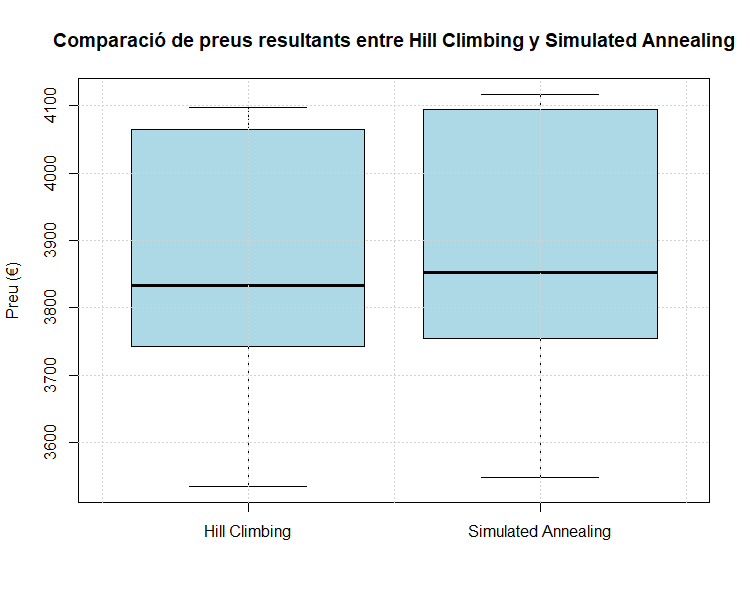
\includegraphics[width=\textwidth]{images/cmpHC_SA_preu.png}
			\caption{Gràfic comparatiu del preu}
			\label{fig:cmpHC_SA_preu}
		\end{minipage} \hfill
		\begin{minipage}{0.45\textwidth}
			\centering
			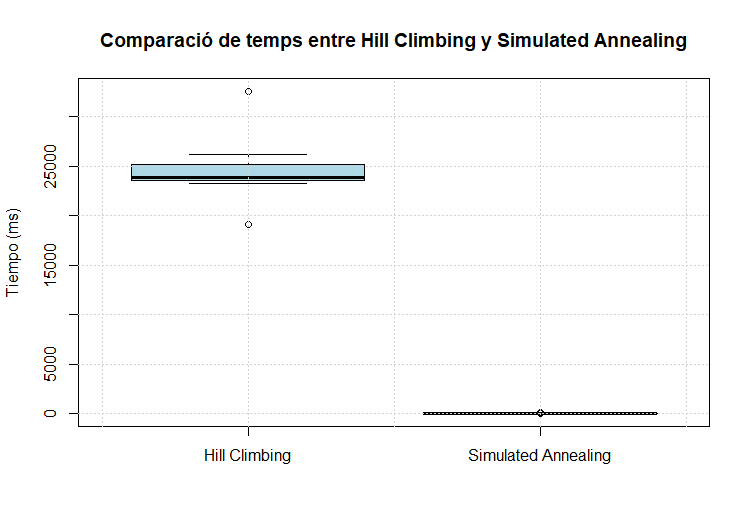
\includegraphics[width=\textwidth]{images/cmpHC_SA_temps.png}
			\caption{Gràfic comparatiu del temps d'execució}
			\label{fig:cmpHC_SA_temps}
		\end{minipage}
	\end{figure}
	
	\begin{table}[H]
		\centering
		\begin{tabular}{|c|c|c|}
			\hline
			\textbf{Algorisme} & \textbf{MitjanaCost} & \textbf{MitjanaTemps(ms)} \\
			\hline
			Hill Climbing & 3863.90 & 24507.40\\
			\hline
			Simulated Annealing & 3883.01 & 52.60\\
			\hline
		\end{tabular}
		\caption{Estadístiques del preu i temps d'execució segons l'algorisme emprat}
		\label{tab:exp10_estadisticas}
	\end{table}

	En les anteriors figures podem observar que el temps d'execució per l'algorisme \textit{Simulated Annealing} és molt menor que per  \textit{Hill Climbing}. Però en canvi, respecte als resultats respecte al cost obtingut, podem veure que el primer algorisme obté lleugerament pitjors resultats, tot i que les diferències tampoc són gaire significatives. \\
	
	Aquests resultats els obtenim malgrat saber que el \textit{Hill Climbing} sol quedar-se atrapat fàcilment en mínims locals, ja que sempre fa passos cap a solucions millors, és a dir, sempre intenta obtenir millors resultats en cada iteració. Això significa que l'algorisme pot trobar una solució que sigui òptima en aquell espai, però que no sigui la millor solució global. \\
	
	En canvi, \textit{Simulated Annealing} té l'avantatge que introdueix un factor d'aleatorietat que li permet escapar d'aquests mínims locals. Inicialment, permet moure's a pitjors solucions amb certa probabilitat, la qual disminueix gradualment a mesura que es "refreda" el procés. Per això, si ajustem correctament els paràmetres, pot arribar a solucions més òptimes que \textit{Hill Climbing}, la qual cosa no ha passat en aquest cas, possiblement perquè el primer algorisme ja ha trobat un bon òptim global. \\
	
	Respecte al temps d'execució, veiem que per una quantitat molt alta d'entrades, el \textit{Simulated Annealing} és més ràpid que el \textit{Hill Climbing}, això pot ser degut a diversos factors. En \textit{Simulated Annealing}, s'estableix un nombre fix d'iteracions (o passos) que defineix el temps d'execució, cosa que permet tenir un límit conegut per endavant. Cada iteració es basa en un pas o salt en l'espai de solucions, la qual cosa evita l'exploració exhaustiva de totes les possibles combinacions de solucions. Així, encara que l'espai de cerca sigui molt gran (com amb un nombre elevat de paquets), l'algorisme es mou de manera controlada i pot trobar una bona solució en un temps raonable sense haver d'explorar tot l'espai.
	Gràcies al procés de refredament, \textit{Simulated Annealing} redueix gradualment la probabilitat d'acceptar solucions pitjors a mesura que avancen les iteracions. A l'inici, l'algorisme es mou de manera més lliure per l'espai de cerca, explorant àmpliament i evitant quedar-se encallat en mínims locals. Aquesta llibertat inicial permet que es recorri una part més gran de l'espai de cerca amb menys passos i, per tant, amb menys temps de computació. A mesura que l'algorisme "refreda", limita les exploracions i es centra en les millors solucions, cosa que li permet convergir ràpidament cap a un punt òptim.
	\textit{Hill Climbing} tendeix a explorar de manera més intensa al voltant d'una solució específica. Això significa que, per cada nova posició, busca la millora més pròxima, cosa que pot resultar ineficient quan l'espai de cerca és gran, el qual creix de forma quadràtica tal com s'ha vist a l'experiment 4 segons creixi el nombre de paquets, i les solucions òptimes estan lluny.   

	
	En conclusió, \textit{Simulated Annealing} és més eficient en espais de cerca grans (nombre de paquets elevats) perquè estableix un nombre fix de passos, controla l'exploració amb el refredament i evita el cost de reavaluar constantment cada possible millora local. Per a problemes amb moltes possibles solucions, aquesta estratègia esdevé més ràpida \textit{Hill Climbing}, obtenint també solucions òtimes semblants a \textit{Hill Climbing}.
	
	\newpage
	\section{Conclusions}
	
	Aquest estudi ha explorat diferents estratègies de cerca local aplicades a un problema d'assignació òptima de paquets amb múltiples criteris. Els resultats experimentals confirmen que l'ús d'operadors específics com el \textit{swap} i \textit{move} i la selecció adequada de paràmetres milloren l'eficiència del sistema. A més, l'algorisme de \textit{Simulated Annealing} ha mostrat avantatges en la cerca d'òptims globals, evitant els mínims locals amb èxit. \\
	
	A més, en aquest estudi s'ha evidenciat la importància de la determinació experimental dels paràmetres en els algorismes de \textit{Hill Climbing} i de \textit{Simulated Annealing} per a aconseguir resultats òptims en la cerca de solucions eficients. S'ha observat que factors com la temperatura inicial, la taxa de refredament i el nombre d'iteracions en el \textit{Simulated Annealing} afecten tant la qualitat de la solució com el temps de convergència. Així, l'ajust experimental dels paràmetres en \textit{Simulated Annealing} permet un equilibri òptim entre exploració i explotació. \\
	
	En futurs treballs, seria interessant investigar l'impacte de combinar altres heurístiques o ajustar més finament els paràmetres de l'algorisme de \textit{Simulated Annealing}. També s'explorarien variacions de pes dels paquets o temps de lliurament més diversificats per analitzar la robustesa del model. A més, una extensió amb algorismes genètics, de satisfacció de restriccions o tècniques de \textit{Machine Learning} podria permetre una adaptació automàtica dels paràmetres en funció de les característiques del problema. \\
	
	En conclusió, aquest estudi ens ha permès consolidar els coneixements adquirits sobre algorismes de cerca local i ens ha dotat de recursos per afrontar problemes complexos, adquirint resultats que poden servir de base per a futures investigacions orientades a millorar l'eficiència i adaptabilitat en aplicacions reals. \\
	
	\section{Coneixements Adquirits}
	En el transcurs del projecte s'han adquirit els següents coneixements:
	
	\begin{itemize}
		\item \textbf{Java amb IntelliJ IDEA}: Desenvolupament de la lògica del projecte amb suport d'un IDE adequat per a projectes complexos.
		\item \textbf{Experimentació amb Algorismes de Cerca Local}: Implementació d'algorismes com \textit{Hill Climbing} (HC) i \textit{Simulated Annealing} (SA) per a l'optimització de solucions.
		\item \textbf{R}: Eina principal per a l'anàlisi de dades experimentals i la seva visualització.
		\item \textbf{\LaTeX}: Redacció del document amb una estructura professional, facilitant una presentació clara i ben organitzada.
		\item \textbf{GitHub}: Gestió i seguiment de versions del projecte, facilitant la col·laboració i organització del codi.
	\end{itemize}
	
	
	
	
	\newpage
	\section{Treball d'Innovació: DeepVariant}
	
	\subsection{Tema}
	Hem escollit DeepVariant, un algorisme de deep learning desenvolupat per Google, que utilitza xarxes neuronals profundes per identificar variants genètiques en dades de seqüenciació de l'ADN. Mitjançant imatges generades a partir de les lectures de seqüència, DeepVariant detecta mutacions petites amb una precisió superior respecte a altres mètodes tradicionals.
	
	\subsection{Responsabilitats d'equip}
	Malgrat que el treball s'està fent col·laborativament i tots els membres del grup participen en totes les tasques, s'ha decidit dividir-ho en tres parts per cercar i aconseguir informació al respecte.
	\begin{itemize}
		\item \emph{Introducció i context}:\\
		Introducció a DeepVariant: què és i per què és rellevant.\\
		Importància de DeepVariant en la detecció de variants genètiques.\\
		Visió general del problema que resol en l'anàlisi de dades de seqüenciació d'ADN.\\
		Per què l'aprenentatge profund és útil en aquest context: beneficis respecte als mètodes tradicionals de detecció de variants (comparació amb altres mètodes).\\
		\textbf{Responsable}: Guillem Cabré\\
		
		\item \emph{Xarxes Neuronals Convolucionals (CNN)}:\\
		Explicació de què són les xarxes neuronals convolucionals (CNNs).\\
		Com s'utilitzen les CNNs en DeepVariant per identificar patrons genètics.\\
		Avantatges de l'ús de CNNs per analitzar dades de seqüenciació d'ADN (perquè reconeixen patrons visuals).\\
		Relació entre les imatges generades per DeepVariant i l'anàlisi de dades genètiques.\\
		\textbf{Responsable}: Hannah Röber\\
		
		\item \emph{Funcionament Pipeline}:\\
		Generació d'imatges a partir de dades de seqüenciació d'ADN.\\
		Com les imatges es passen per la xarxa neuronal convolucional per ser classificades.\\
		Processos d'inferència: com es decideix quina variant està present (substitució, inserció, deleció).\\
		Entrenament de la xarxa neuronal amb dades genètiques.\\
		Presa de decisions sobre la presència de variants genètiques i avantatges de precisió i fiabilitat.\\
		\textbf{Responsable}: Carla Cordero\\
	\end{itemize}
	
	
	
	\subsection{Referències}
	
	\begin{itemize}
		\item GitHub: \url{https://github.com/google/deepvariant} Rellevància: és el repositori oficial que inclou codi, instruccions de instal·lació, i scripts per executar DeepVariant, i, a més, models d'entrenament i eines d'avaluació. També porta a altres documents com: \url{https://google.github.io/deepvariant/posts/2020-02-20-looking-through-deepvariants-eyes/} Data d'accés: 13 d'octubre de 2024.
		\item \emph{Creating a universal SNP and small indel variant caller with deep neural networks}:
		Rellevància: Base teòrica de DeepVariant i explicació de l'ús de xarxes neuronales.
		Data d'accés: 13 d'octubre de 2024.
		Enllaç: \url{https://doi.org/10.1101/092890}
		i \url{https://www.biorxiv.org/content/biorxiv/suppl/2016/12/19/092890.DC2/092890-1.pdf}
		\item Zou J, Huss M, Abid A, Mohammadi P, Torkamani A, Telenti A. \emph{A primer on deep learning in genomics}. Nat Genet. 2019 Jan;51(1):12-18. doi: 10.1038/s41588-018-0295-5. Epub 2018 Nov 26. PMID: 30478442; PMCID: PMC11180539. Rellevància: proveeix una base en la recerca en l'anàlisi de dades genòmiques utilitzant xarxes neuronals convolucionals, arquitectura de la qual està formada DeepVariant. Data d'accés: 20 d'octubre de 2024.
		\item \emph{Deep learning for genomics: A concise overview}:
		Rellevància: Proporciona una visió general sobre l'aplicació d'aprenentatge profund en la genòmica, incloent exemples pràctics i metodologia.
		Data d'accés: 28 d'octubre de 2024.
		Enllaç: \url{https://pmc.ncbi.nlm.nih.gov/articles/PMC7481958/}
		\item \emph{Deep learning in bioinformatics and genomics}:
		Rellevància: Explora les aplicacions de l'aprenentatge profund en bioinformàtica, amb un enfocament en la seva importància per a l'anàlisi de dades genòmiques.
		Data d'accés: 28 d'octubre de 2024.
		Enllaç: \url{https://www.nature.com/articles/nbt.4235}
		\item Lin, YL., Chang, PC., Hsu, C. et al. \textit{Comparison of GATK and DeepVariant by trio sequencing}. Sci Rep 12, 1809 (2022). \url{https://doi.org/10.1038/s41598-022-05833-4} Rellevància: per observar la comparació en precisió i velocitat entre DeepVariant amb una altra eina que fa un treball similar com GATK \textit{Genome Analysis Toolkit}. Data d'accés: 17 d'octubre de 2024.
		\item Taedong Yun, Helen Li, Pi-Chuan Chang, Michael F Lin, Andrew Carroll, Cory Y McLean, \textit{Accurate, scalable cohort variant calls using DeepVariant and GLnexus}, Bioinformatics, Volume 36, Issue 24, December 2020, Pages 5582–5589, \url{https://doi.org/10.1093/bioinformatics/btaa1081} Rellecvància: una altra comparació entre DeepVariant i \textit{GLNexus} per observar el rendiment de DeepVariant en comparació amb altres eines. Data d'accés: 17 d'octubre de 2024.
	\end{itemize}
	
	\subsection{Dificultats}
	\begin{itemize}
		\item \emph{Accés a referències}: Alguns articles rellevants requereixen subscripcions per poder obtenir informació detallada.
		\item \emph{Informació tècnica}: Hem hagut de fer un sobreesforç perquè es requereix d'un mínim de coneixements sobre l'ADN per entendre la proposta.
	\end{itemize}
	
	\newpage
	\section{Annex}
	\label{sec:annex}
	
	\subsection*{Enllaç al Codi}
	
	El codi font i documentació addicional del projecte estan disponibles al repositori de GitHub. Podeu accedir-hi mitjançant el següent enllaç:
	
	\href{https://github.com/Willyllem88/IA-LocalSearch}{GitHub - IA-LocalSearch} \\
	
	En aquest repositori, a més del codi, es proporcionen instruccions de compilació i execució, així com les \textit{spreadsheets} dels experiments, els \textit{scripts} en \texttt{R} i els gràfics resultants d'aquests.

	\subsection*{Documentació de classes Java}
	
	En el desenvolupament de la pràctica s'han utilitzat diverses classes Java. A continuació, es descriu cadascuna d'elles:
	
	\begin{itemize}
		\item \texttt{Paquet}: Representa un paquet individual, incloent informació com el pes i la prioritat. Aquesta classe s'encarrega de gestionar les propietats de cada paquet i proporciona mètodes per accedir a aquesta informació.
		\item \texttt{Paquets}: Genera una estructura amb tots els paquets que s'han de lliurar. Rep com a paràmetres el nombre de paquets i la llavor per a la generació aleatòria.
		\item \texttt{Transporte}: Representa les ofertes de transport disponibles. Rep com a paràmetres l'estructura de paquets, una proporció de pes i una llavor per a la generació aleatòria.
		\item \texttt{Oferta}: Inclou la informació sobre les ofertes de transport, com el pes màxim i el preu per quilogram.
	\end{itemize}
	
	\subsection*{Eines estadístiques per analitzar els resultats}
	
	Per realitzar una anàlisi completa dels resultats dels experiments, és útil emprar eines estadístiques que facilitin la comparació entre diferents mètodes. Algunes suggeriments inclouen:
	
	\begin{itemize}
		\item \textbf{Mitjana i desviació estàndard:} Per determinar l'estabilitat i consistència dels resultats en diferents rèpliques.
		\item \textbf{Diagrames de caixa (Box plots):} Útils per visualitzar la dispersió dels resultats i detectar possibles valors atípics.
	\end{itemize}
	
	\subsection*{Consideracions finals sobre el disseny d'experiments}
	
	En l'experimentació, s'han pres diverses decisions metodològiques amb l'objectiu d'obtenir resultats significatius:
	
	\begin{itemize}
		\item \textbf{Elecció de la llavor:} S'ha utilitzat una llavor específica per garantir que tots els experiments fossin reproduïbles.
		\item \textbf{Nombre de rèpliques:} Cada experiment s'ha replicat almenys deu vegades per calcular valors mitjans fiables.
		\item \textbf{Visualització de resultats:} S'han emprat gràfics per facilitar la interpretació visual de les dades obtingudes en cada experiment.
	\end{itemize}
	
\end{document}